\documentclass[11pt, aspectratio=169]{beamer}
%\documentclass{beamer}
\setbeamertemplate{navigation symbols}{}
\usetheme{Boadilla}
\usecolortheme{beaver}
\usepackage{caption}


\usepackage{tikz} 
\usepackage{adjustbox}
\usepackage{multicol}


\usepackage{graphicx}
\usepackage{subcaption}
\usepackage{algorithm}
\usepackage{algpseudocode}
%\usepackage[noend]{algorithmic}
\usepackage{amsmath}
\usefonttheme{professionalfonts}
\usepackage{helvet}
\renewcommand{\familydefault}{\sfdefault}
%\renewcommand{\figurename}{Gambar}
\usepackage{hanging}
\usepackage{lipsum}
\usepackage{listings}
\newcommand\blfootnote[1]{%
  \begingroup
  \renewcommand\thefootnote{}\footnote{#1}%
  \addtocounter{footnote}{-1}%
  \endgroup
}
\setbeamertemplate{caption}{\insertcaption}

\setbeamertemplate{footnote}{\tiny \hangpara{1em}{1}\makebox[1em][l]{\insertfootnotemark}\footnotesize\insertfootnotetext\par}
\hyphenation{}

\usepackage{ragged2e}
\renewcommand\thempfootnote{\arabic{mpfootnote}}



%=======================================================
%KETERANGAN FRAME
\title[DVB-T2 LDPC Codes]{Study on LDPC Codes for Indonesia Digital Video Broadcasting Terrestrial 2nd Generation (DVB-T2)}
%\subtitle{Avoiding Common Mistakes}
\author[Citra Yasin Akbar Fadhlika]{ \vspace{-0.1in}
%
\includegraphics[height=0.35in]{gambarafa/logoSOFTT}
\hspace{0.05in}

\includegraphics[height=0.25in]{gambarafa/adwitech}
\hspace{0.05in}

\includegraphics[height=0.25in]{gambarafa/telu.jpg}\\ \quad \\ \small Citra Yasin Akbar Fadhlika\\1101164109\\
\vspace*{-0.02in}
		Supervisor:  Dr. Eng. Khoirul Anwar, S. T., M. Eng.\\
		Co-supervisor:  Budi Prasetya, S.T., M. T.\\
		\vspace{-0.21in}
}
\vspace{-0.5in}
\institute[] {  The Center for Advanced Wireless Technologies (AdWiTech), Telkom University,\\
Jl. Telekomunikasi No. 1, Terusan Buah Batu, Bandung, 40257 Indonesia.\\
E-mail: \{\textit{citrayaf@student., anwarkhoirul@, budiprasetya@ \}telkomuniversity.ac.id}
\blfootnote{\tiny{This research is supported in part by the World Class Research Grant for T3LESDM-Net, 2019--2021.\\
		Some part of this thesis have been published on Symposium of Future Telecommunication Technologies (SOFTT) 2019}}
\vspace{-0.21in}
}
%
\vspace{-0.21in}
\date[January $7^{th}, 2020$]{\footnotesize Presented at Final Defense of Bachelor's Thesis\\
 Bandung, Indonesia }


%			LET'S START YEYEYEYYEYE
%========================================================
% Let's get started the document
\begin{document}
\justifying

\begin{frame}
  \titlepage
\end{frame}
\begin{frame}{Outline}
  \tableofcontents
  % You might wish to add the option [pausesections]
\end{frame}
%-----------------------------------------------------------------------


%=======================================================
%=======================================================
\section{Problems and Motivations}
%--------------------------------------
\begin{frame}{Problems and Motivations}
%--------------------------------------

%\begin{figure}
%\centering
%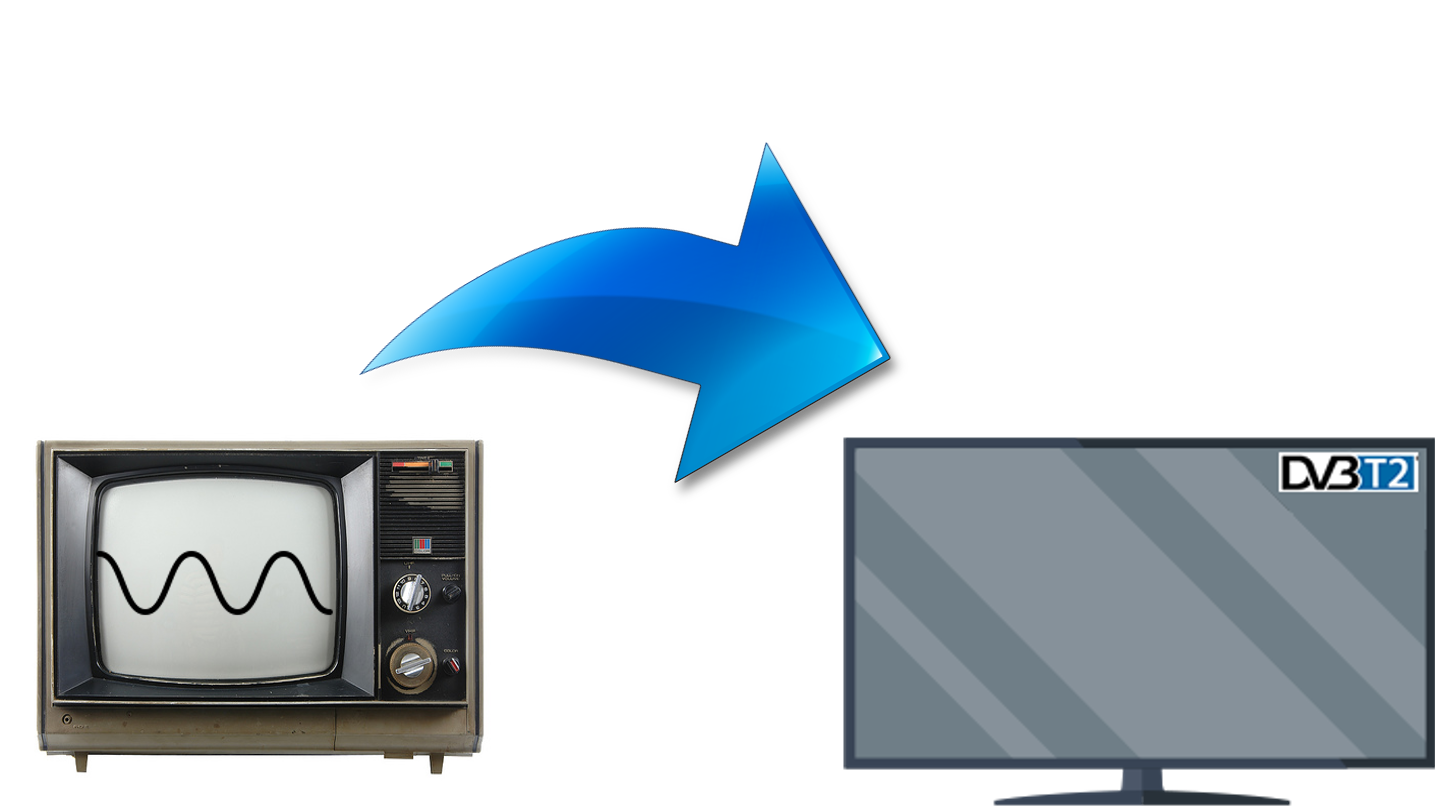
\includegraphics[scale=0.15]{gambarafa/tvdig}
%%\caption{Indonesia Digital Television Standard Migration.}
%\label{downlink} 
%\end{figure}
\begin{figure}
\centering
%	\hspace{ -in}
\vspace{-.95cm}
\begin{minipage}{.5\linewidth}
	\hspace{1cm}
	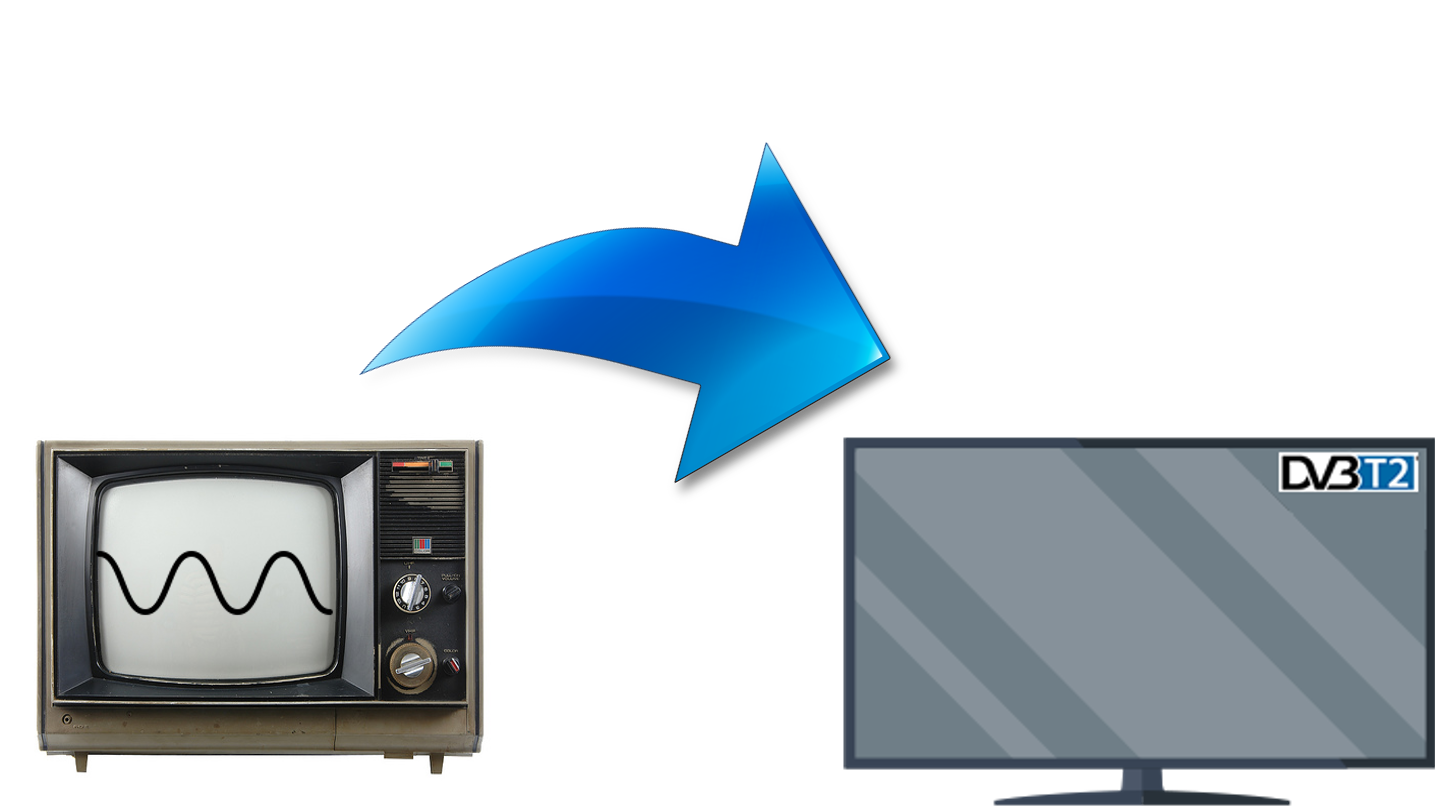
\includegraphics[width=2.5in]{gambarafa/tvdig}
	\vspace{1cm}
	
	%		\center (a)
\end{minipage}
\hfill 	
\hspace{ -1in}
\begin{minipage}{.5\linewidth}
	\hspace{2.3cm}
	\includegraphics[width=3in]{PEG/TannerH}
	
	\vspace{-0.5cm}
	%		\center (b)
\end{minipage}
\hfill
%	\begin{minipage}{.5\linewidth}
%		\hspace{-0.5cm}
%		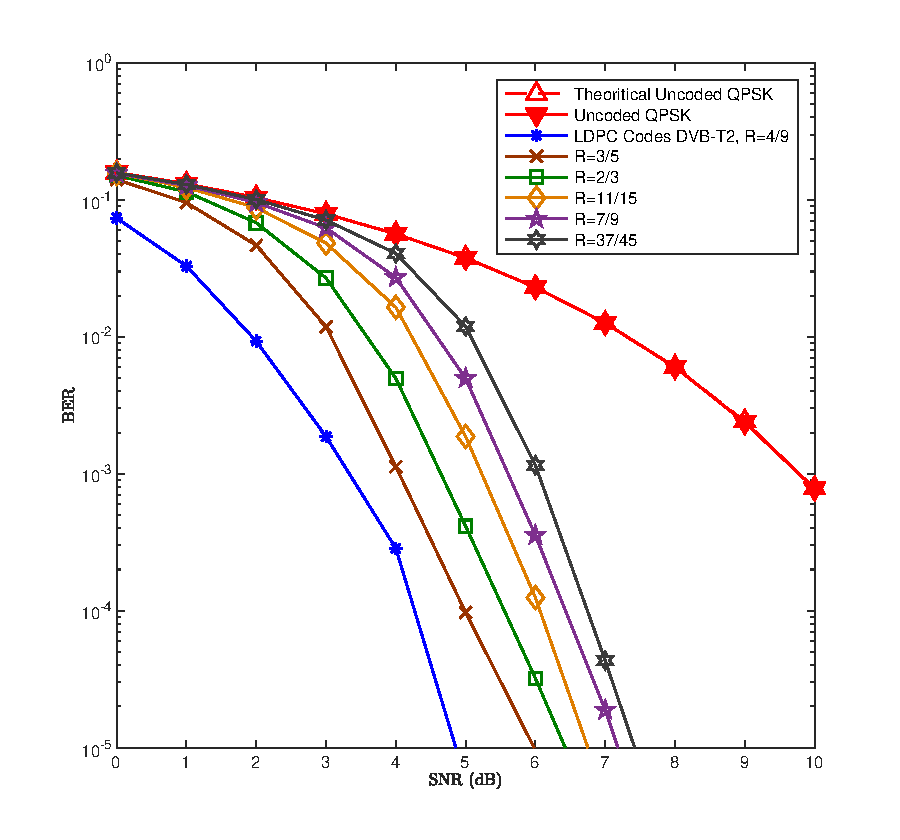
\includegraphics[width=3in]{hasilpegawgnfix.pdf}
%		\vspace{-1.5cm}
%		\center (c)
%	\end{minipage}
%	\hspace{-0.1 in}
%	\begin{minipage}{.5\linewidth}
%		%		\hspace{2.25 cm}
%		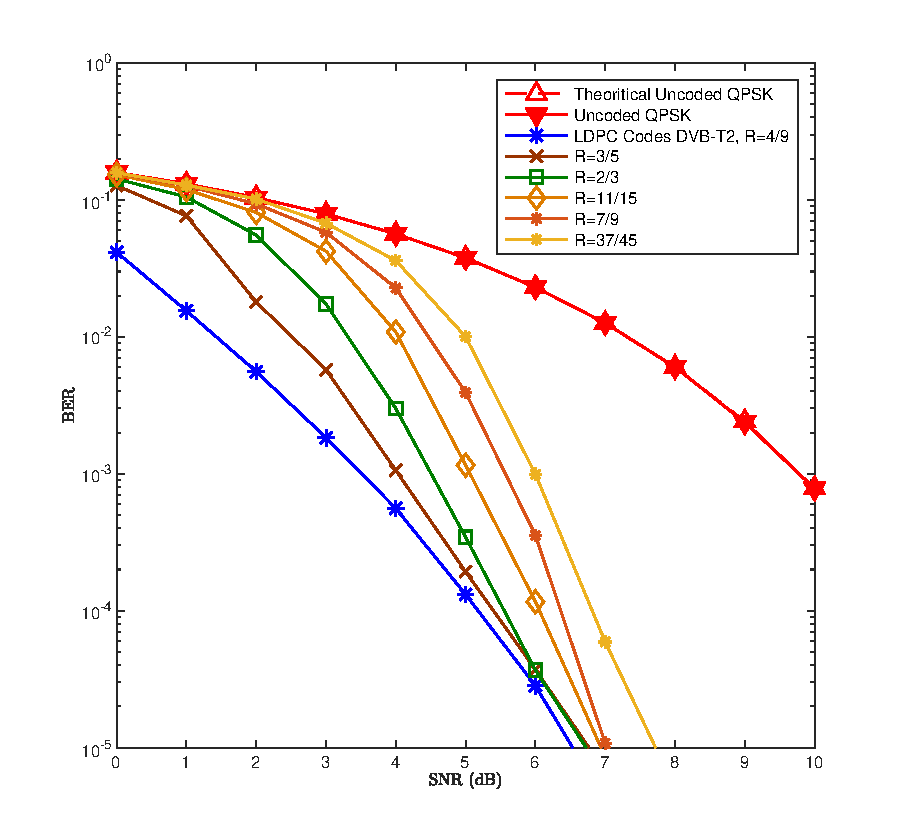
\includegraphics[width=3in]{hasilpegawgnfixLDGM.pdf}
%		\vspace{-1.5cm}
%		\center \hspace*{0.75cm}(d)
%	\end{minipage}
%	\caption {Kinerja BER LDPC \textit{codes} DVB-T2 dengan: (a) $N_{LDPC}=270$ menggunakan metode \textit{downscaled}, (b) $N_{LDPC}=16200$, (c) $N_{LDPC}=270$ menggunakan PEG dengan IRA, dan (d) $N_{LDPC}=270$ menggunakan PEG dengan LDGM pada kanal AWGN .}
\label{gambar: awgnhasil}
\end{figure}
\vspace{-35pt}
\begin{itemize}
	
	
	
	
	
\justifying
\item The unavailability of lower band spectrum in Indonesia, because the frequency usage of traditional Indonesia Television. 
\item DVB-T2 standard is used as the Indonesia terrestrial digital television standard having possibility to free up some frequency band.  \blfootnote{\tiny{Minisitry of Communications and Informatics Indonesia Regulation Number: 05/PER/M.KOMINFO/2/2012.}}
\item The suitable Low Density Parity Check (LDPC) codes for Indonesia channel model leading to an optimal performances is absence.
\begin{enumerate}
	\item Degree distribution.
	\item Constructing structure.
\end{enumerate}
\end{itemize}
\end{frame}



\section{Basic Theory}
%=======================================================
\begin{frame}{Low Density Parity Check (LDPC) Codes}
	%--------------------------
\vspace{-0.2 cm}
	\begin{figure}
		\centering
		%	\hspace{ -in}
		\vspace{-0.25cm}
		\begin{minipage}{.5\linewidth}
			\hspace{-0.25cm}
			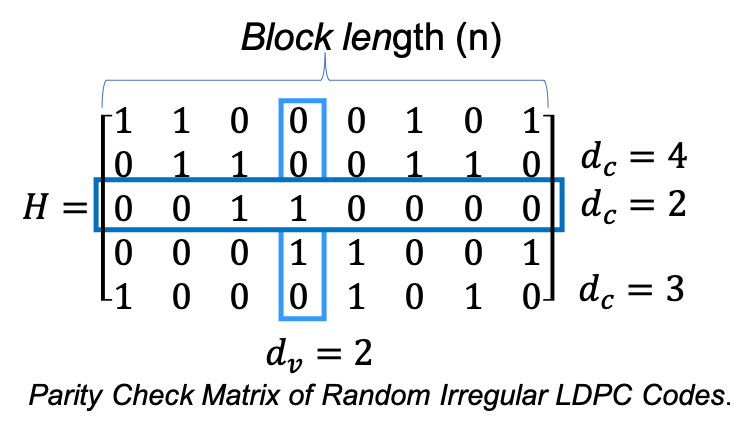
\includegraphics[width=2.5in]{PEG/matrixirre.png}
			\vspace{-0.5cm}
			
			%		\center (a)
		\end{minipage}
		\hfill 	
		\hspace{ -1in}
		\begin{minipage}{.5\linewidth}
			\hspace{0.75cm}
			\includegraphics[width=3.65in]{PEG/TannerH}
			
			\vspace{-0.5cm}
			%		\center (b)
		\end{minipage}
		\hfill
		%	\begin{minipage}{.5\linewidth}
		%		\hspace{-0.5cm}
		%		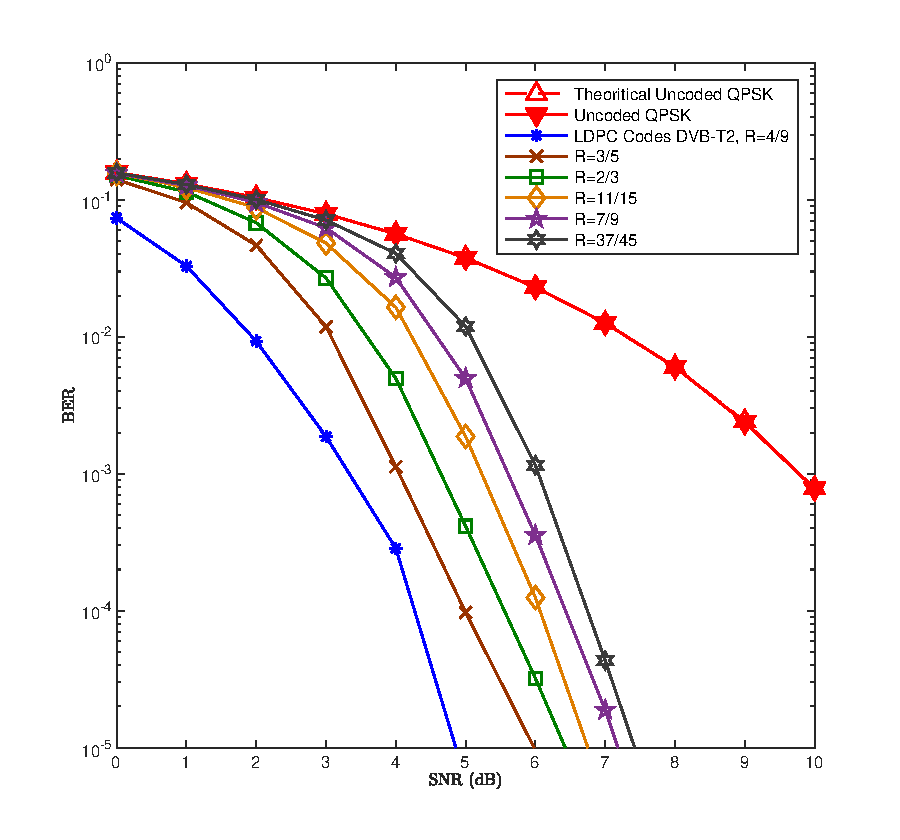
\includegraphics[width=3in]{hasilpegawgnfix.pdf}
		%		\vspace{-1.5cm}
		%		\center (c)
		%	\end{minipage}
		%	\hspace{-0.1 in}
		%	\begin{minipage}{.5\linewidth}
		%		%		\hspace{2.25 cm}
		%		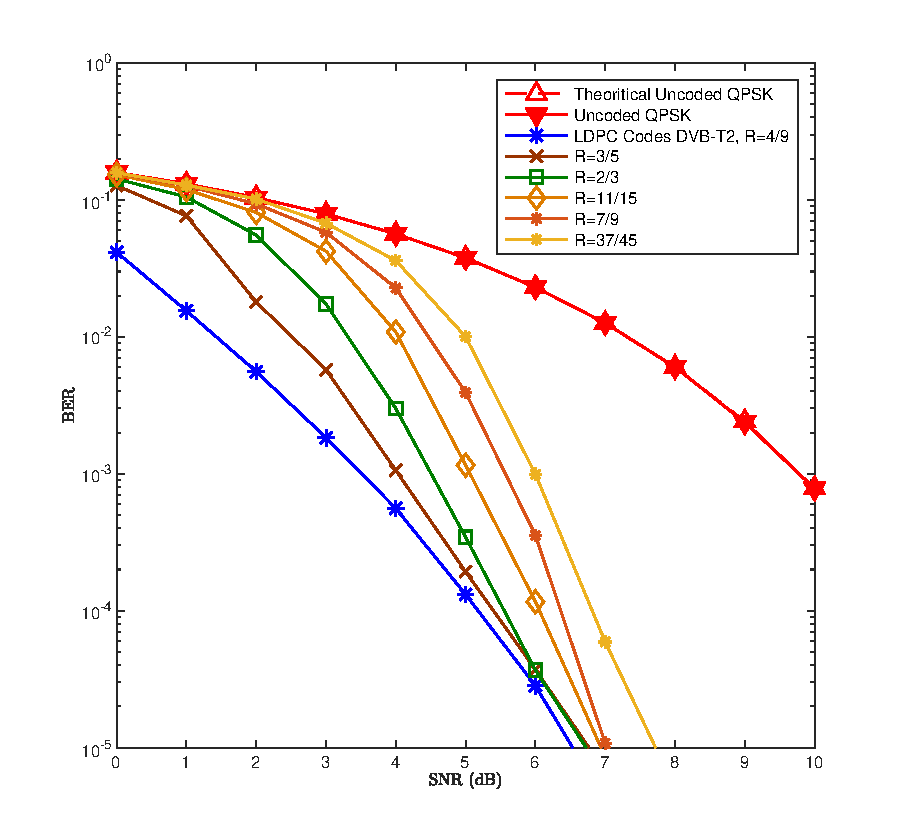
\includegraphics[width=3in]{hasilpegawgnfixLDGM.pdf}
		%		\vspace{-1.5cm}
		%		\center \hspace*{0.75cm}(d)
		%	\end{minipage}
		%	\caption {Kinerja BER LDPC \textit{codes} DVB-T2 dengan: (a) $N_{LDPC}=270$ menggunakan metode \textit{downscaled}, (b) $N_{LDPC}=16200$, (c) $N_{LDPC}=270$ menggunakan PEG dengan IRA, dan (d) $N_{LDPC}=270$ menggunakan PEG dengan LDGM pada kanal AWGN .}
		\label{gambar: awgnhasil}
	\end{figure}
%		\begin{figure}
%					\centering %taro di tengah
%					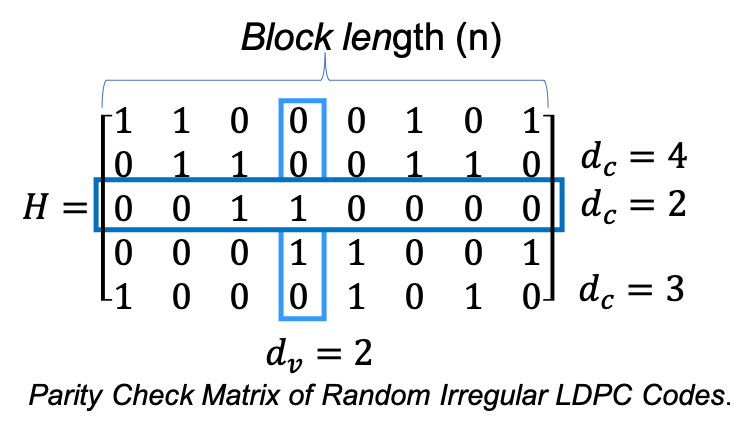
\includegraphics[scale=0.45]{PEG/matrixirre.png}
%					%\caption{Bipartite graph of parity check matrix $\mathbf{H}$.}
%					\label{bipartitH} 
%				\end{figure}
%			\begin{figure}
%				\centering 
%				\includegraphics[scale=0.6]{PEG/TannerH}
%				\centering 
%				\label{sistemmodelMQCLDPC} %~\ref{kucing}
%			\end{figure}
\vspace{0.5cm}
	\footnotesize{
		\begin{itemize}
			\item LDPC codes have been proved to be capable of closely approaching the channel capacity.\\
			\item LDPC codes are codes specified by a matrix containing mostly 0’s and only a small number of 1’s.
			\blfootnote{\tiny Todd K. Moon,”Error Correcting Coding Mathematical methods and Algorithms”, p. 634-679, 2005.
			} \\
%			\item \textit{Parity check matrix LDPC codes $\mathbf{H}$}\\
%			
%			\begin{itemize}
%				\footnotesize{
%					\item[$\checkmark$] Block lenght $n$
%					\item[$\checkmark$] Variable node degree $d_v$
%					\item[$\checkmark$] Check node degree $d_c$    
%			} \end{itemize}
			\item Parity check matrix of LDPC codes $\mathbf{H}$ can be represent as a graph using Tanner graph and degree distribution.\blfootnote{\tiny R. Tanner, "A recursive approach to low complexity codes," in IEEE Transactions on Information Theory, vol. 27, no. 5, pp. 533-547, September 1981.
			} 
				\begin{eqnarray}
			\Lambda (x) &=& x^2, \\
			\Omega(x) &=& \frac{1}{5}x^{2}+\frac{2}{5}x^{3}+\frac{2}{5}x^{4}.
			\end{eqnarray}
			%\item Low latency channel coding and low complexity.
		\end{itemize}
	}
%	\vspace{-40pt}
%	\begin{columns}
%		\column{.4\textwidth}
%%		\begin{eqnarray}
%%%		\mathbf{G}&=&[I_k\; P]%,\\
%%		%\mathbf{H}&=&[-P^T\; I_{n-k}],\\
%%		%\mathbf{G}\cdot \mathbf{H}^T&=&0.
%%		\end{eqnarray}
%		
%		\column{.6\textwidth}
%		\centering
%		\begin{figure}
%			\centering %taro di tengah
%			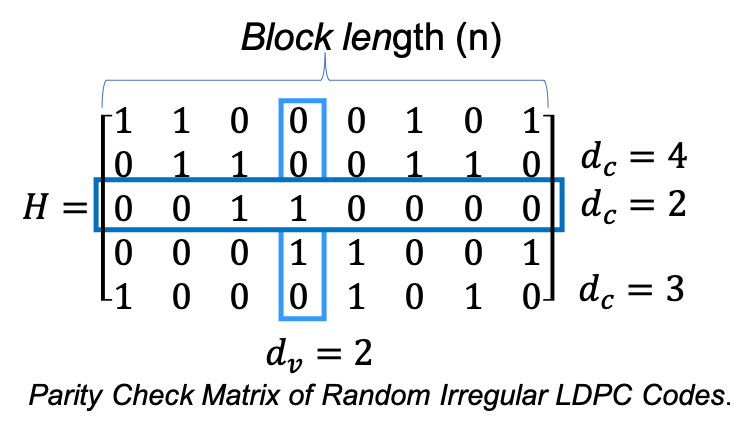
\includegraphics[scale=0.45]{PEG/matrixirre.png}
%			%\caption{Bipartite graph of parity check matrix $\mathbf{H}$.}
%			\label{bipartitH} 
%		\end{figure}
%		
%	\end{columns}
\end{frame}


%\begin{frame}{Tanner Graph}
%	%--------------------------
%	\vspace{-1cm}
%	\begin{figure}
%		\centering 
%		\includegraphics[scale=0.6]{PEG/TannerH}
%		\centering 
%		\label{sistemmodelMQCLDPC} %~\ref{kucing}
%	\end{figure}
%	
%	\begin{itemize}
%		%\item SIMPLE : Small block size less than 2000
%		\item Parity check matrix of LDPC codes $\mathbf{H}$ can be represent as a graph using Tanner graph, Tanner graph consist of two set node.\blfootnote{\tiny R. Tanner, "A recursive approach to low complexity codes," in IEEE Transactions on Information Theory, vol. 27, no. 5, pp. 533-547, September 1981.
%		} 
%		\begin{eqnarray}
%	\Lambda (x) &=& x^2, \\
%	\Omega(x) &=& \frac{1}{5}x^{2}+\frac{3}{5}x^{3}+\frac{1}{5}x^{4}.
%	\end{eqnarray}
%		
%%		\item Matriks \textit{parity check} LDPC \textit{codes} $H$ dapat direpresentasikan menggunakan Tanner \textit{graph} dengan dua set \textit{node}.\footnote[1]{\tiny R. Tanner, "A recursive approach to low complexity codes," in IEEE Transactions on Information Theory, vol. 27, no. 5, pp. 533-547, September 1981.
%%		} 
% 		\item Edges between variable nodes and check node will connected if only if
% 		\begin{equation}
% 		H_{i,j}=1,
% 		\end{equation}
% 		with $i$ is for variable node or column of matrix and $j$ is for check node or row of matrix.
%
% 
%%		\item Garis (\textit{edge}) antara \textit{variable nodes} dengan \textit{check nodes} terhubung apabila 
%%		\begin{equation}
%%		H_{i,j}=1,
%%		\end{equation}
%%		dengan $i$ adalah \textit{variable node} ke-$i$ dan $j$ adalah \textit{check node} ke-$j$.
%		
%		
%		%\item The systems use narrowband system with single carrier transmission.
%		%\item Channels are Additive White Gaussian Noise (AWGN) and frequency-flat Rayleigh fading.
%		%\item Perfect channel synchronization and estimation.
%		%\begin{itemize}
%		%\item Matrix Generator $G$ in encoder.
%		%\item Parity Check Matrix $H$ in decoder. 
%		%\end{itemize}
%		%\vspace{-0.35cm}
%		%\begin{eqnarray}
%		%\mathbf{G}\cdot \mathbf{H}^T&=&0.
%		%\end{eqnarray}
%	\end{itemize}
%	
%	\vspace{-20pt}
%	%\begin{figure}
%	%\centering 
%	%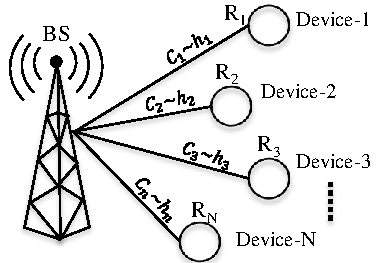
\includegraphics[scale=0.85]{pics/downlink2.pdf}
%	%\caption{Configuration of downlink IoT wireless communication systems.}
%	%\label{massiveiot} %~\ref{kucing}
%	%\end{figure}
%	
%\end{frame}



%\begin{frame}{Girth}
%	%--------------------------
%	\begin{figure}
%		\centering 
%		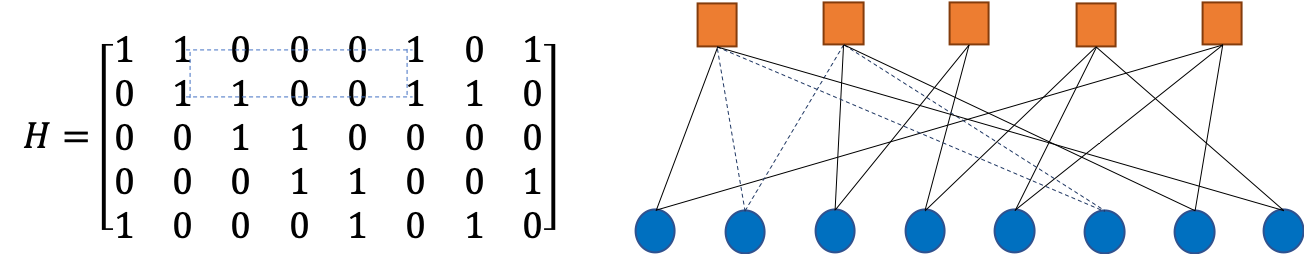
\includegraphics[scale=0.6]{PEG/GirthH}
%		\centering 
%	\end{figure}
%	\begin{itemize}
%		
%		\item Girth is the shortest cycle of LDPC codes that affect the LDPC \textit{codes} performances, this cycle can be seen from Tanner graph of LDPC \textit{codes}.\blfootnote{\tiny J. Fan and Y. Xiao, "A Method of Counting the Number of Cycles in LDPC Codes," 2006 8th international Conference on Signal Processing, Beijing, 2006, pp.}  
%%		\item \textit{Girth} adalah panjang siklus terpendek dalam sebuah Tanner \textit{graph} yang menjadi hal penting dalam menentukan kinerja LDPC \textit{codes}.
%%		\item Local girth is the shortest cycle from one variable node in a LDPC codes Tanner graph.
%
%
%
%%				\item \textit{Girth} lokal pun terbentuk dari siklus per \textit{node} pada sebuah Tanner \textit{graph} LDPC \textit{codes}.  
%		\item Small girth will leave a bad effect on the LDPC codes decoders, because they affect the independence of extrinsic information which exchanged in iterative decoding.\blfootnote{\tiny M. Sipser and D. A. Spielman, "Expander codes," in IEEE Transactions on Information Theory, vol. 42, no. 6, pp. 1710-1722, Nov. 1996.}  
%%		\item Terjadinya \textit{girth} kecil akan memberikan efek buruk pada LDPC codes, karena mengurangi kinerja dari \textit{extrinsic information} dalam proses \textit{iterative decoding}.\footnote[2]{\tiny M. Sipser and D. A. Spielman, "Expander codes," in IEEE Transactions on Information Theory, vol. 42, no. 6, pp. 1710-1722, Nov. 1996.}  
%		
%	\end{itemize}
%	
%	.
%	
%\end{frame}



%\begin{frame}{EXIT Chart}
%\begin{columns}
%	\column{.37 \textwidth}
%	
%
%	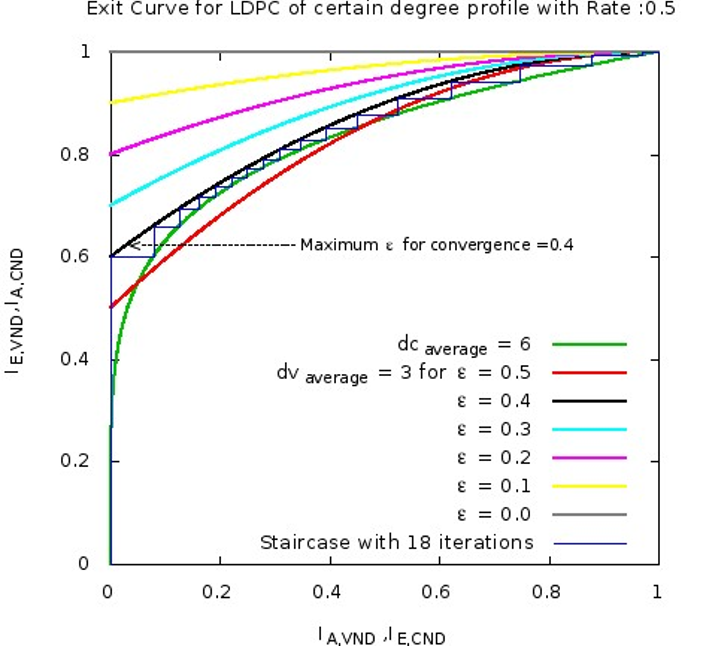
\includegraphics[scale=.55]{gambarafa/lol}
%
%	
%
%	
%\column{.63 \textwidth}
%	\begin{itemize}
%		\justifying
%%		\item \textbf{EX}trinsic \textbf{I}nformation \textbf{T}ransfer (EXIT) Chart introduced by Stephan ten Brink, it's a method used to evaluate performance of any iterative decoder and giving a feedback on required number of iterations to reach successful decoding.
%		\footnotesize
%		\item The EXIT chart is plotted as the a priori mutual information $I_A$ before message is decoded and the extrinsic mutual information $I_E$ after decoding.
%%		\item The output extrinsic mutual information of a variable node and check node denoted as $I_{E,VND}$ and $I_{E,CND}$, for the input a priori mutual information of a variable node and check node denoted as $I_{A,VND}$ and $I_{A,CND}$.
%
%\begin{equation}
%I_{E,V}\! =\! \sum_i \mathcal{F}_i^\Lambda { J\left( \sqrt{(d_{V_i}\!-\!1)[J^{-1}(I_{A,V})]^2 + [J^{-1}(I_{A_{ch}})]^2 }  	\right)
%%		\!+\! [J^{-1}(I_{A,V}^{ext})]^2}
% }
%\label{eq:I_E_V_int}
%\end{equation} 
%
%\begin{equation}
%I_{E,C} = 1-\sum_i \mathcal{F}_i^\Omega J\left( \sqrt{(d_{C_i}-1)[J^{-1}(1-I_{A,C})]^2}\right)
%\end{equation}
%
%	\end{itemize}
%	
%\end{columns}
%
%\end{frame}

%\section{Proses \textit{Encoding} dan \textit{Decoding} pada QC-LDPC codes}
%\begin{frame}
%	\tableofcontents[currentsection,currentsubsection]
%\end{frame}


%\begin{frame}{\textit{Encoding} and \textit{Decoding} of LDPC \textit{Codes}}
%	\begin{columns}
%		\vspace{-10pt}
%		\column{.5\textwidth}
%		\begin{figure}
%			\centering
%			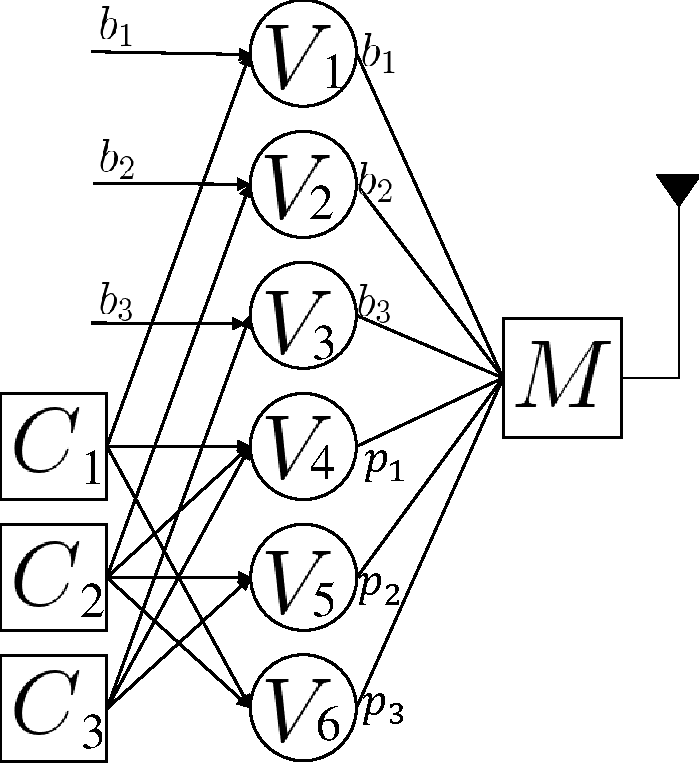
\includegraphics[width=.5\textwidth]{sumber/encoder2.pdf}
%			%\caption{Contoh grafik Tanner matriks generator LDPC \textit{codes}.}
%		\end{figure}
%		\footnotesize{ Generator matrix $ \mathbf{G} $ is sets of check node $ \mathbf{C} $, interleaver $\Pi_x$, and variable node $ \mathbf{V} $ on the transmitter. So the codeword $\mathbf{c}$ can be achived $\mathbf{c}=\mathbf{bG}$.}
%		
%		\column{.5\textwidth}
%		\vspace{-10pt}
%		\begin{figure}
%			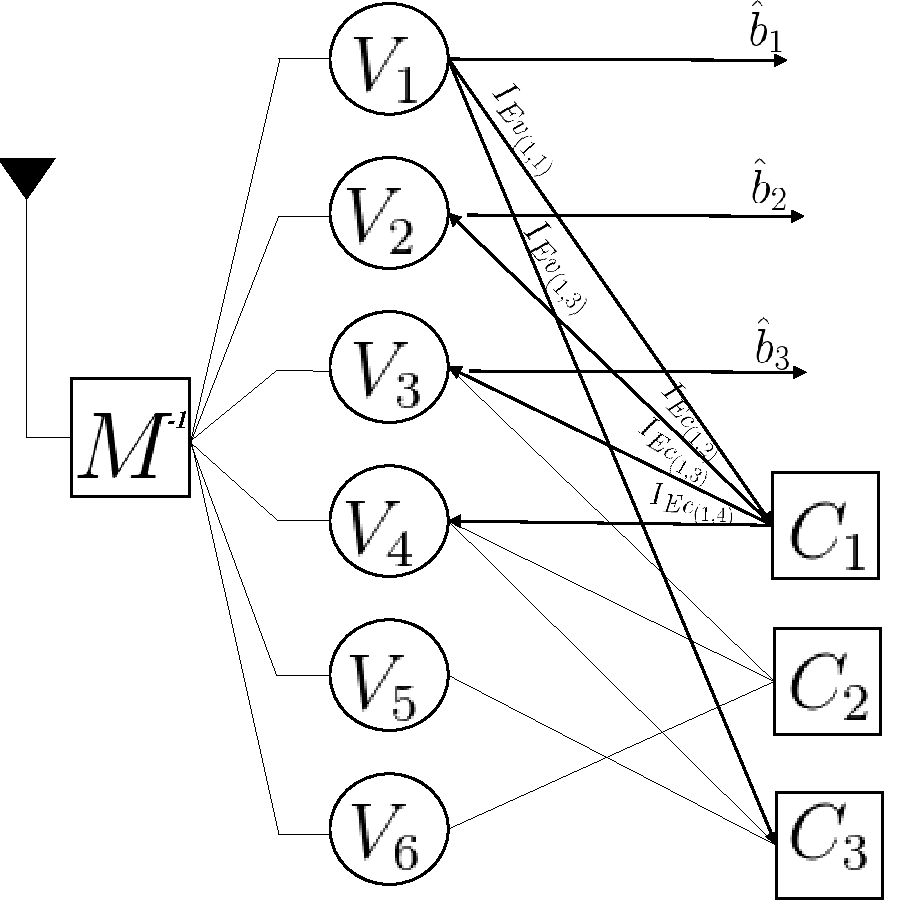
\includegraphics[width=.59\textwidth]{sumber/Decoder.pdf}
%		\end{figure}
%		\footnotesize{Parity check matrix  $\mathbf{H}$ is a decoder set in receiver. This thesis use sum product algorithm (SPA) for the iterative decoding of LDPC codes.
%%			LDPC \textit{decoder} melakukan \textit{iterative} $\mathbf{V-C-V}$ \textbf{sum product algorithm}.
%		}
%		% LLR menunjukkan probabilitas suatu variabel memiliki nilai tertentu.
%	\end{columns}
%\end{frame}
%=======================================================
\section{System Model of DVB-T2}

%--------------------------


%--------------------------
\begin{frame}{System Model of DVB-T2}
%--------------------------

	\begin{figure}
	\centering
%	\hspace{ tin}
	%		\vspace{-0.25cm}
	\begin{minipage}{.5\linewidth}
		\hspace{0.5cm}
		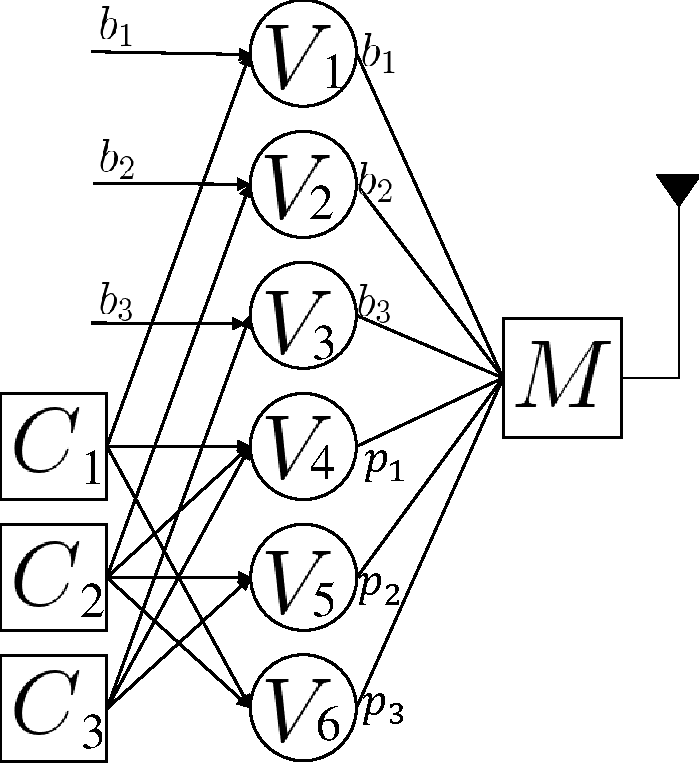
\includegraphics[width=1in]{sumber/encoder2.pdf}
		\vspace{-0.5cm}
		
		%		\center (a)
	\end{minipage}
	\hfill 	
	\hspace{ -2in}
	\begin{minipage}{.5\linewidth}
%		\hspace{ 2cm}
		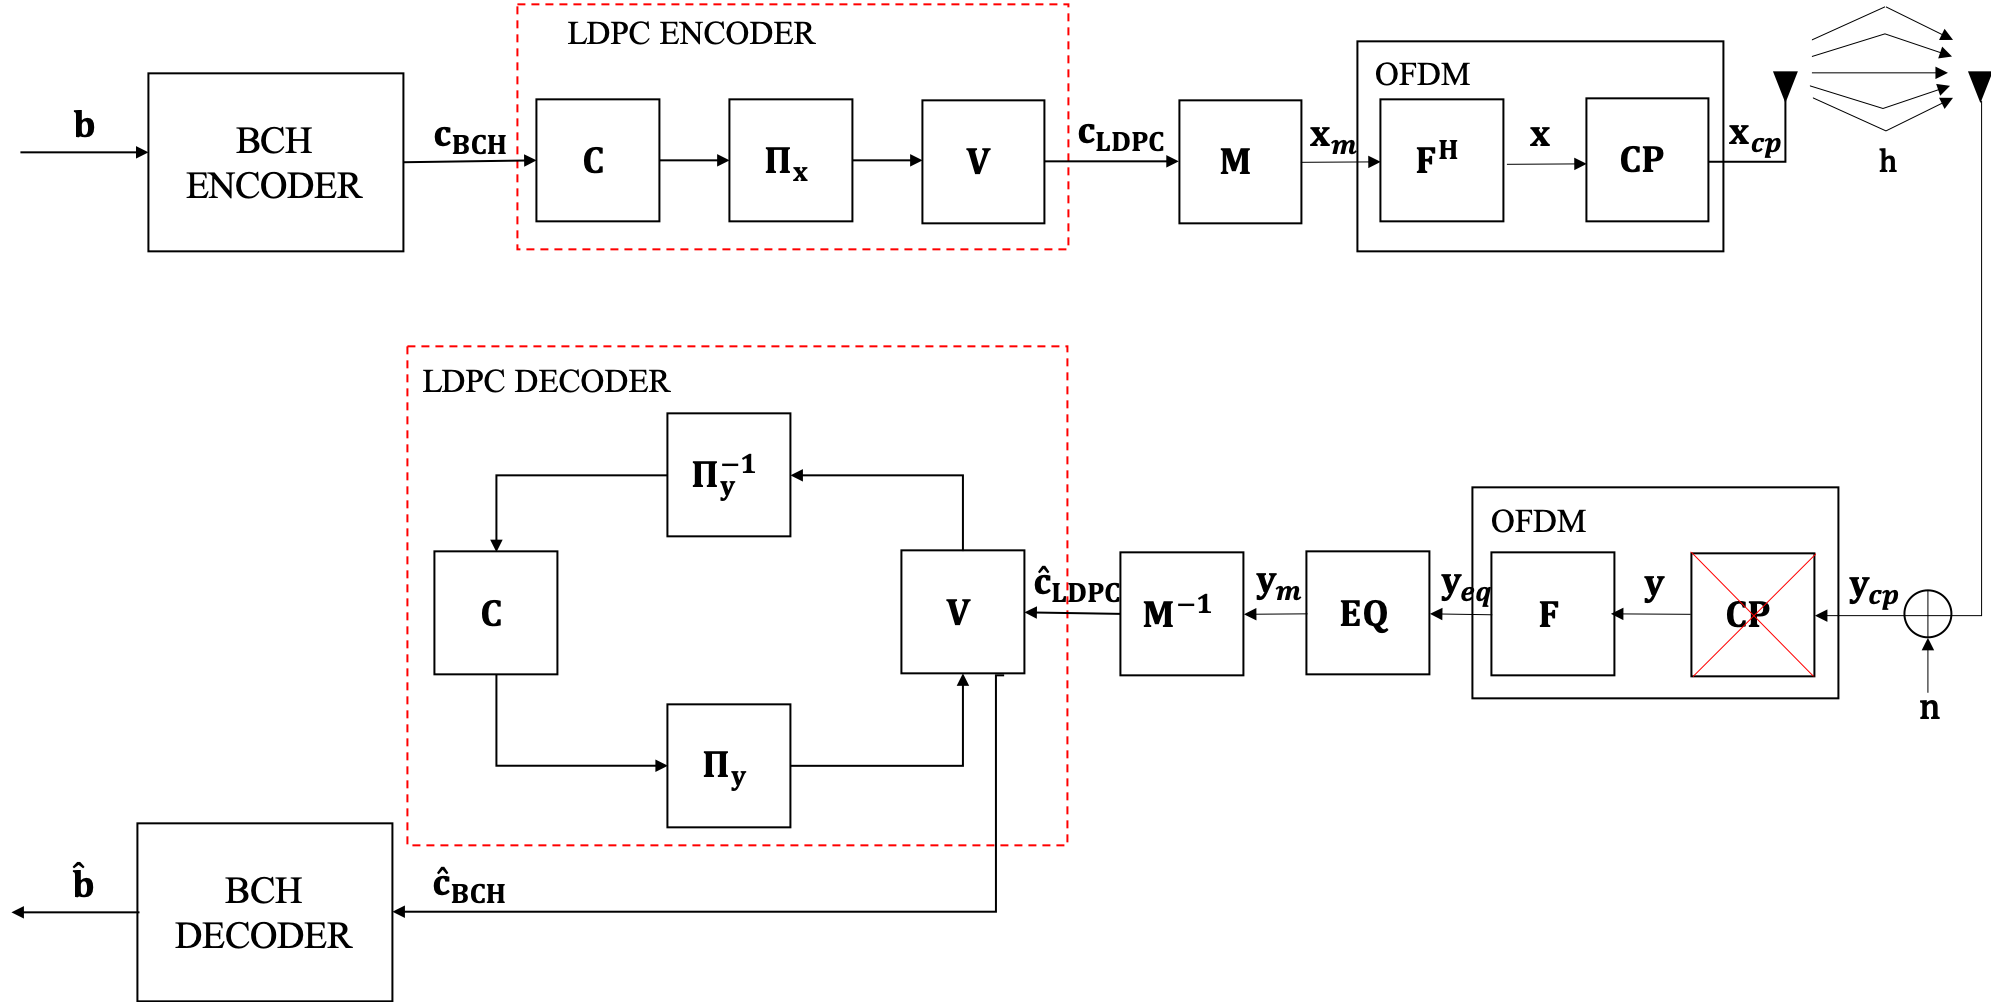
\includegraphics[width=3in]{gambarafa/sistemmo}
		
		\vspace{0.5cm}
		%		\center (b)
	\end{minipage}
	\hfill
	\hspace{ -2in}
	\begin{minipage}{.5\linewidth}
		\hspace{4.5 cm}
		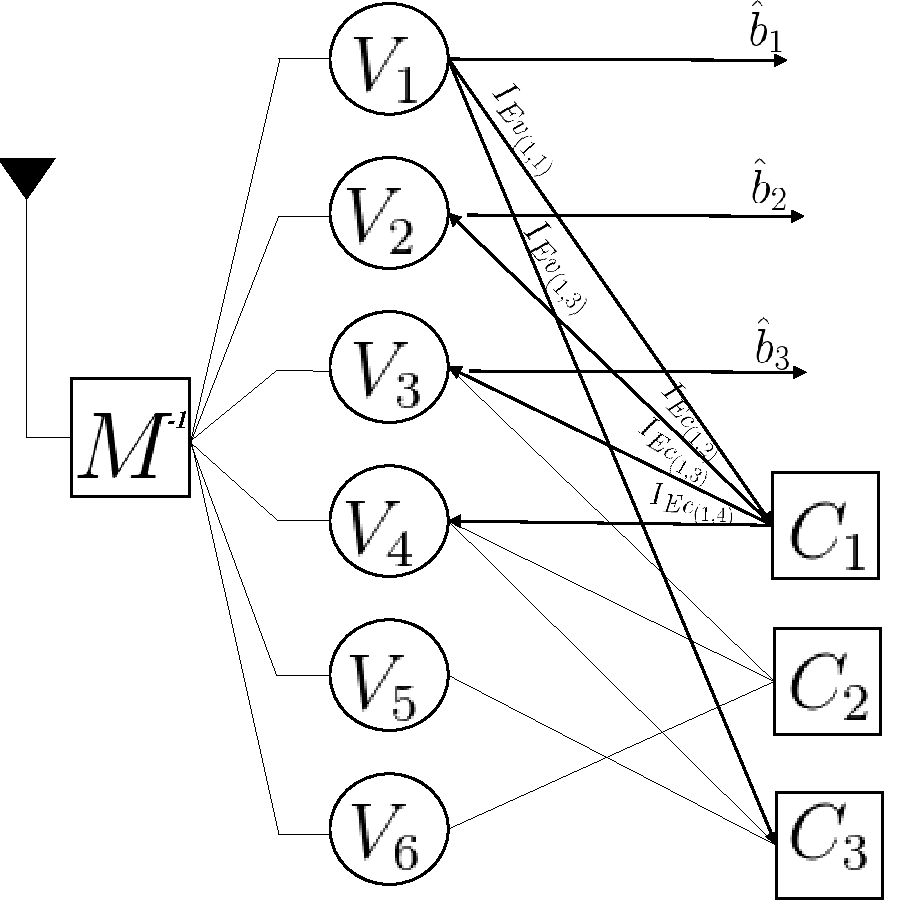
\includegraphics[width=1in]{sumber/Decoder.pdf}
		\vspace{-0.9cm}
		%			\center (c)
	\end{minipage}
	%	\begin{minipage}{.5\linewidth}
	%		\hspace{-0.5cm}
	%		\includegraphics[width=3in]{hasilawgnfix.pdf}
	%		\vspace{-1.5cm}
	%		\center (c)
	%	\end{minipage}
	%	\hspace{-0.1 in}
	%	\begin{minipage}{.5\linewidth}
	%		%		\hspace{2.25 cm}
	%		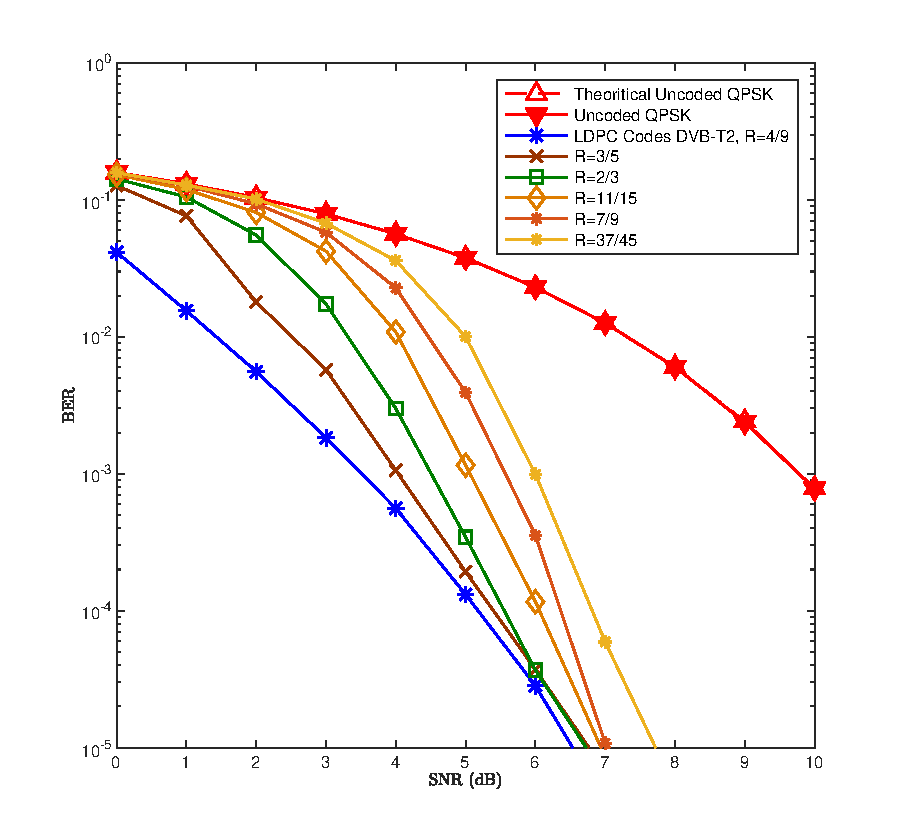
\includegraphics[width=3in]{hasilpegawgnfixLDGM.pdf}
	%		\vspace{-1.5cm}
	%		\center \hspace*{0.75cm}(d)
	%	\end{minipage}
	%	\caption {Kinerja BER LDPC \textit{codes} DVB-T2 dengan: (a) $N_{LDPC}=270$ menggunakan metode \textit{downscaled}, (b) $N_{LDPC}=16200$, (c) $N_{LDPC}=270$ menggunakan PEG dengan IRA, dan (d) $N_{LDPC}=270$ menggunakan PEG dengan LDGM pada kanal AWGN .}
	\label{gambar: awgnhasil}
\end{figure}

%\vspace{-10pt}
%		\begin{figure}
%	\centering
%	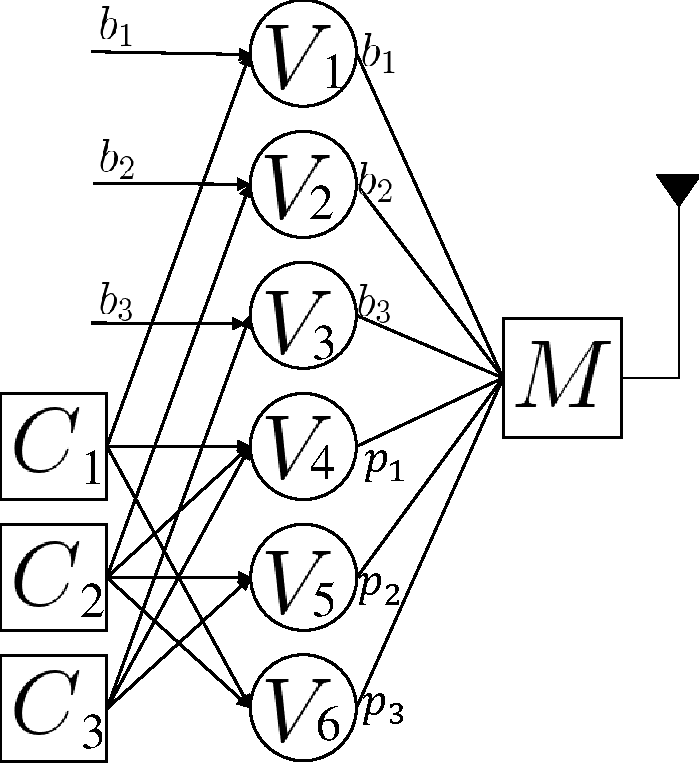
\includegraphics[width=.15\textwidth]{sumber/encoder2.pdf}
%	%\caption{Contoh grafik Tanner matriks generator LDPC \textit{codes}.}
%\end{figure}
%\begin{figure}
%\centering 
%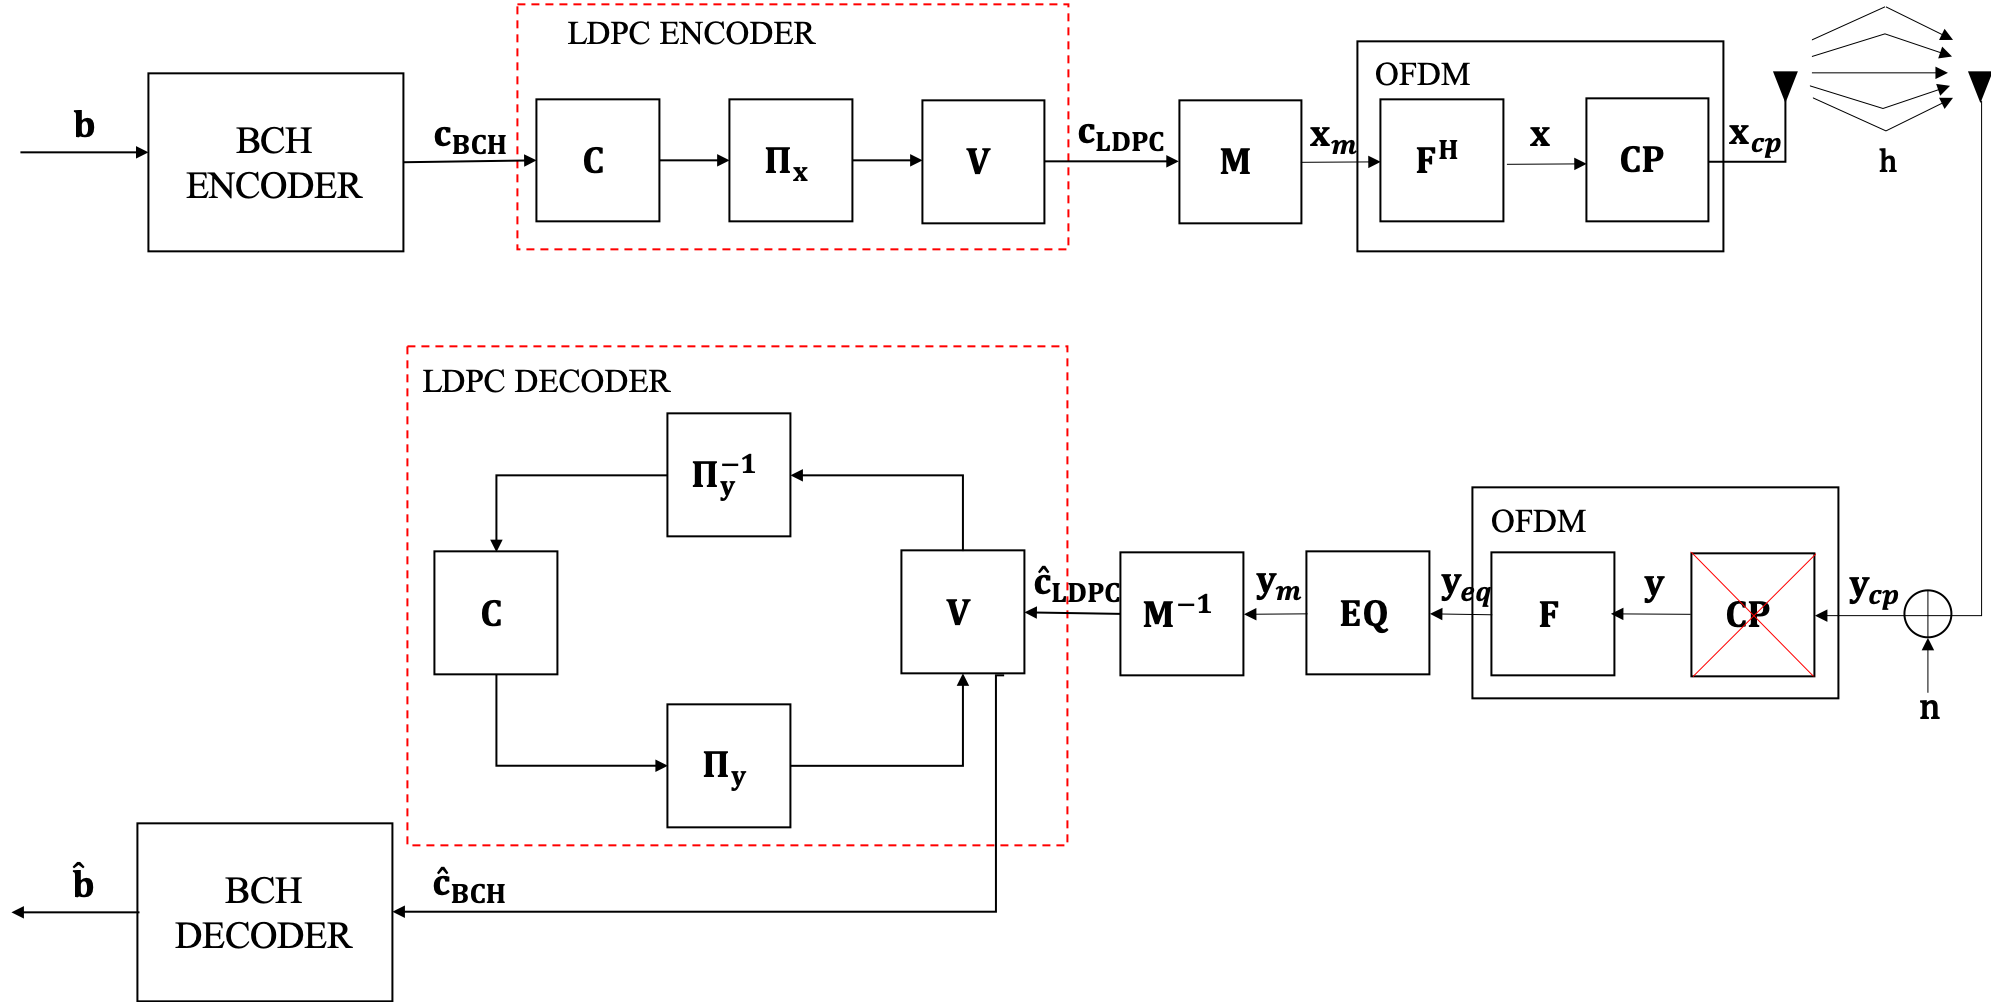
\includegraphics[scale=0.25]{gambarafa/sistemmo}
%\label{sistemmodelMQCLDPC} %~\ref{kucing}
%\end{figure}
\vspace{-5pt}
\begin{itemize}
\item The structure of LDPC encoder and decoder are adapted from ETSI TS 102 831 V1.2.1.
\item The modulation $\mathbf{M}$ is Quadrature Phase Shift Keying (QPSK). 
\item This thesis consider multipath channel $\mathbf{h}$ using Bandung DVB-T2 channel model.\blfootnote{\tiny{D. Fitriyani, K. Anwar, and D. M. Saputri, "Study on Radio Frequency Profile of Indonesia Digital Television DVB-T2 for Urban Areas", in ICONISTECH 2019.}}
\end{itemize}
%\begin{columns}
%\hspace{10pt}
%\column{.4\textwidth}
%\small{$\mathbf{b}$ : information bits\\
%$\mathbf{C}$ : check nodes\\
%$\Pi$ : interleaver\\
%$\mathbf{V}$ : variable nodes\\
%$\mathbf{c_{BCH}}$ : BCH codewords\\
%$\mathbf{c_{LDPC}}$ : LDPC codewords\\
%$\mathbf{M}$ : modulator\\
%$\mathbf{x_{cp}}$ : transmit symbols\\
%}
%\column{.4\textwidth}
%\small{$\mathbf{h}$ : Bandung channel\\
%$\mathbf{n}$ : noise\\
%$\mathbf{y_{cp}}$ : received symbols\\
%$\mathbf{M^{-1}}$ : demodulator\\
%%$L_{ch}$ : LLR channel\\
%%$I_E$ : extrinsic information\\
%%$I_A$ : mutual information\\
%$\mathbf{\hat{c}_{LDPC}}$ : estimated LDPC codewords\\
%$\mathbf{\hat{c}_{BCH}}$ : estimated BCH codewords\\
%$\mathbf{\hat{b}}$ : estimated bits information\\}
%\end{columns}
\end{frame}
%=======================================================
%=======================================================
\begin{frame}{DVB-T2 LDPC Codes}
%--------------------------

\vspace{-1cm}


\begin{columns}
	\begin{column}{0.5\textwidth}
		
		\begin{figure}
			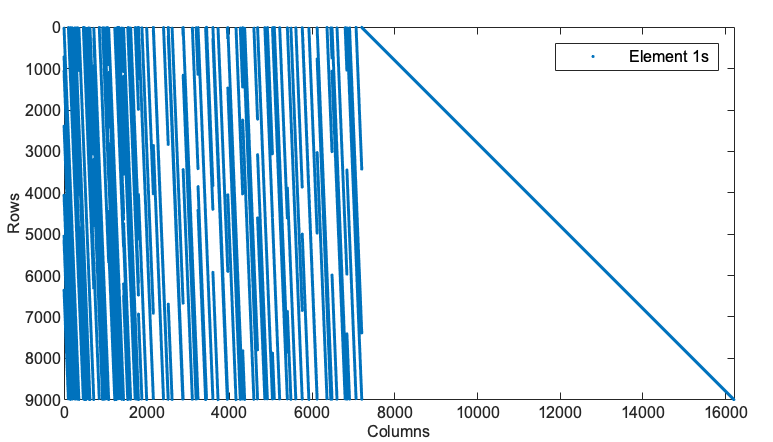
\includegraphics[scale=0.5]{gambarafa/hs(1-2)-2}
			
		\end{figure}
		
	\end{column}
	\begin{column}{0.55\textwidth}  
		\begin{center}
			{\footnotesize
				\begin{table}
							\begin{adjustbox}{width=0.8\textwidth , totalheight=\textheight-2\baselineskip,keepaspectratio}
				\renewcommand{\figurename}{Table}
				\centering 
				\label{table:dvb-t2lite}
				\begin{tabular}{|c|c|c|c|c|c|c|c|}
					\hline
					\multicolumn{2}{|c|}{Code rate} & \multicolumn{6}{c|}{Column weight}    \\ \hline
					$R_n$  & $R_e$  & 13   & 12   & 8    & 3     & 2    & 1 \\ \hline
					1/2           & 4/9             &      &      & 1800 & 5400  & 8999 & 1 \\ \hline
					3/5           & 3/5             &      & 3240 &      & 6480  & 6479 & 1 \\ \hline
					2/3           & 2/3             & 1080 &      &      & 9720  & 5399 & 1 \\ \hline
					3/4           & 11/15           &      & 360  &      & 11520 & 4319 & 1 \\ \hline
					4/5           & 7/9             &      &      &      & 12600 & 3599 & 1 \\ \hline
					5/6           & 37/45           & 360  &      &      & 12960 & 2879 & 1 \\ \hline
				\end{tabular}
				\end{adjustbox}
				
				
				
				
			\end{table}
			}
		\end{center}
	\end{column}
\end{columns}



%\begin{figure}
%\centering 
%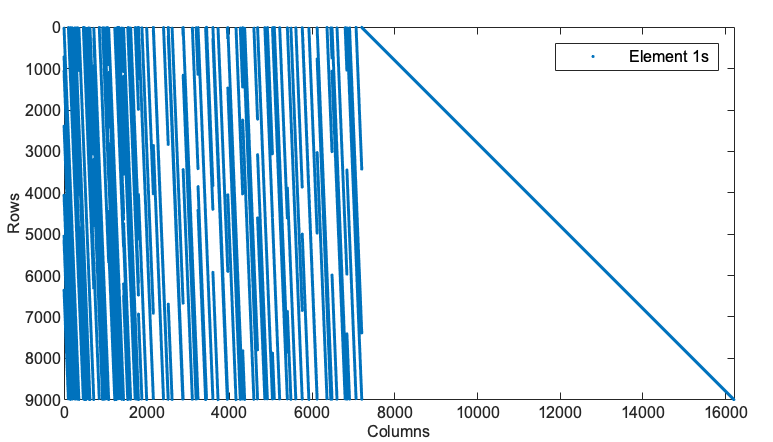
\includegraphics[scale=0.4]{gambarafa/hs(1-2)-2}
%\centering 
%\label{sistemmodelMQCLDPC} %~\ref{kucing}
%\end{figure}
%
%	\begin{table}
%	\renewcommand{\figurename}{Table}
%	\centering 
%	\label{table:dvb-t2lite}
%	\begin{tabular}{|c|c|c|c|c|c|c|c|}
%		\hline
%		\multicolumn{2}{|c|}{Code rate} & \multicolumn{6}{c|}{Column weight}    \\ \hline
%		$R_n$  & $R_e$  & 13   & 12   & 8    & 3     & 2    & 1 \\ \hline
%		1/2           & 4/9             &      &      & 1800 & 5400  & 8999 & 1 \\ \hline
%		3/5           & 3/5             &      & 3240 &      & 6480  & 6479 & 1 \\ \hline
%		2/3           & 2/3             & 1080 &      &      & 9720  & 5399 & 1 \\ \hline
%		3/4           & 11/15           &      & 360  &      & 11520 & 4319 & 1 \\ \hline
%		4/5           & 7/9             &      &      &      & 12600 & 3599 & 1 \\ \hline
%		5/6           & 37/45           & 360  &      &      & 12960 & 2879 & 1 \\ \hline
%	\end{tabular}
%
%
%
%	
%	
%\end{table}

\begin{itemize}
%\item SIMPLE : Small block size less than 2000
\item DVB-T2 LDPC codes according to ETSI TS 102 831 V1.2.1 have block-length $N_{LDPC}=16200$ and $N_{LDPC}=64800$.

\item LDPC codes with $N_{LDPC}=16200$ have code rates $R=\left \{ \frac{4}{9}, \frac{3}{5}, \frac{2}{3},\frac{11}{15},\frac{7}{9},\frac{37}{45} \right \}$.

\item The parity check matrices of DVB-T2 LDPC codes $\mathbf{H}$ are constructed according to the value from addresses parity bit accumulator and column weight distribution of each code rate.
\blfootnote{\tiny{ETSI, Digital Video Broadcasting (DVB); Frame Structure Channel Coding and Modulation for a Second Generation Digital Terrestrial Television Broadcasting System (DVB-T2), 1st ed., ETSI, July 2015.}}
%\item We proposed DVB-T2 LDPC codes with $N_{LDPC}=16200$ having code rates $R=\frac{4}{9}$.
%\item The systems use narrowband system with single carrier transmission.
%\item Channels are Additive White Gaussian Noise (AWGN) and frequency-flat Rayleigh fading.
%\item Perfect channel synchronization and estimation.
%\begin{itemize}
%\item Matrix Generator $G$ in encoder.
%\item Parity Check Matrix $H$ in decoder. 
%\end{itemize}
%\vspace{-0.35cm}
%\begin{eqnarray}
%\mathbf{G}\cdot \mathbf{H}^T&=&0.
%\end{eqnarray}
\end{itemize}

\vspace{-20pt}







%\begin{figure}
%\centering 
%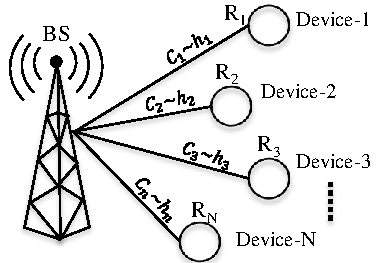
\includegraphics[scale=0.85]{pics/downlink2.pdf}
%\caption{Configuration of downlink IoT wireless communication systems.}
%\label{massiveiot} %~\ref{kucing}
%\end{figure}

\end{frame}
%%--------------------------
%\begin{frame}{Basic Theory}

%--------------------------
%\begin{frame}{The Addresses of Parity Bit Accumulator}
%	%--------------------------
%\vspace{-0.35cm}
%\begin{columns}
%	\column{.45 \textwidth}
%	\begin{table}[tb]
%		\begin{adjustbox}{width=0.8\textwidth , totalheight=\textheight-2\baselineskip,keepaspectratio}
%			\begin{tabular}{|l|l|l|lllll}
%				\hline
%				\multicolumn{1}{|c|}{20} & \multicolumn{1}{c|}{712}  & \multicolumn{1}{c|}{2386} & \multicolumn{1}{c|}{6354} & \multicolumn{1}{c|}{4061} & \multicolumn{1}{c|}{1062} & \multicolumn{1}{c|}{5045} & \multicolumn{1}{c|}{5158} \\ \hline
%				\multicolumn{1}{|c|}{21} & \multicolumn{1}{c|}{2543} & \multicolumn{1}{c|}{5748} & \multicolumn{1}{c|}{4822} & \multicolumn{1}{c|}{2348} & \multicolumn{1}{c|}{3089} & \multicolumn{1}{c|}{6328} & \multicolumn{1}{c|}{5876} \\ \hline
%				\multicolumn{1}{|c|}{22} & \multicolumn{1}{c|}{926}  & \multicolumn{1}{c|}{5701} & \multicolumn{1}{c|}{269}  & \multicolumn{1}{c|}{3693} & \multicolumn{1}{c|}{2438} & \multicolumn{1}{c|}{3190} & \multicolumn{1}{c|}{3507} \\ \hline
%				\multicolumn{1}{|c|}{23} & \multicolumn{1}{c|}{2802} & \multicolumn{1}{c|}{4520} & \multicolumn{1}{c|}{3577} & \multicolumn{1}{c|}{5324} & \multicolumn{1}{c|}{1091} & \multicolumn{1}{c|}{4667} & \multicolumn{1}{c|}{4449} \\ \hline
%				\multicolumn{1}{|c|}{24} & \multicolumn{1}{c|}{5140} & \multicolumn{1}{c|}{2003} & \multicolumn{1}{c|}{1263} & \multicolumn{1}{c|}{4742} & \multicolumn{1}{c|}{6497} & \multicolumn{1}{c|}{1185} & \multicolumn{1}{c|}{6202} \\ \hline
%				0                        & 4046                      & 6934                      &                           &                           &                           &                           &                           \\ \cline{1-3}
%				1                        & 2855                      & 66                        &                           &                           &                           &                           &                           \\ \cline{1-3}
%				2                        & 6694                      & 212                       &                           &                           &                           &                           &                           \\ \cline{1-3}
%				3                        & 3439                      & 1158                      &                           &                           &                           &                           &                           \\ \cline{1-3}
%				4                        & 3850                      & 4422                      &                           &                           &                           &                           &                           \\ \cline{1-3}
%				5                        & 5924                      & 290                       &                           &                           &                           &                           &                           \\ \cline{1-3}
%				6                        & 1467                      & 4049                      &                           &                           &                           &                           &                           \\ \cline{1-3}
%				7                        & 7820                      & 2242                      &                           &                           &                           &                           &                           \\ \cline{1-3}
%				8                        & 4606                      & 3080                      &                           &                           &                           &                           &                           \\ \cline{1-3}
%				9                        & 4633                      & 7877                      &                           &                           &                           &                           &                           \\ \cline{1-3}
%				10                       & 3884                      & 6868                      &                           &                           &                           &                           &                           \\ \cline{1-3}
%				11                       & 8935                      & 4996                      &                           &                           &                           &                           &                           \\ \cline{1-3}
%				12                       & 3028                      & 764                       &                           &                           &                           &                           &                           \\ \cline{1-3}
%				13                       & 5988                      & 1057                      &                           &                           &                           &                           &                           \\ \cline{1-3}
%				14                       & 7411                      & 3450                      &                           &                           &                           &                           &                           \\ \cline{1-3}
%			\end{tabular}
%		\end{adjustbox}
%		
%	\end{table}
%	\column{.55 \textwidth}
%	\begin{itemize}
%		
%		\item The parity check matrix of DVB-T2 LDPC codes with $N_{LDPC}=16200$ constructed from each the addresses of parity bit accumulator for every code rate.
%		\item Column from the addresses of parity bit accumulator table is expressed amount of variable node degree, while the row is expressed the amount of variable node with every row expressed 360 node.
%		
%	\end{itemize}
%	%Where $q$ is amount of column and $j$ is amount of row from addresses of parity bit accumulators, $s_f$ is the scaling factor, $P$ is amount of $N-K$ in the original DVB-T2 LDPC codes, and the range of k is $1< k\leq \left ( 360/s_f \right )$. 
%\end{columns}
%	
%	\blfootnote{\tiny{ETSI, Digital Video Broadcasting (DVB); Frame Structure Channel Coding and Modulation for a Second Generation Digital Terrestrial Television Broadcasting System (DVB-T2), 1st ed., ETSI, July 2015.}}
%	
%\end{frame}
%
%
%%--------------------------
%\begin{frame}{The Parity Check Matrices }
%	%--------------------------
%	\vspace{-0.5cm}
%	\begin{table}
%		\renewcommand{\figurename}{Table}
%		\centering 
%		\label{table:dvb-t2lite}
%		\begin{tabular}{|c|c|c|c|c|c|c|c|}
%			\hline
%			\multicolumn{2}{|c|}{Code rate} & \multicolumn{6}{c|}{Column weight}    \\ \hline
%			$R_n$  & $R_e$  & 13   & 12   & 8    & 3     & 2    & 1 \\ \hline
%			1/2           & 4/9             &      &      & 1800 & 5400  & 8999 & 1 \\ \hline
%			3/5           & 3/5             &      & 3240 &      & 6480  & 6479 & 1 \\ \hline
%			2/3           & 2/3             & 1080 &      &      & 9720  & 5399 & 1 \\ \hline
%			3/4           & 11/15           &      & 360  &      & 11520 & 4319 & 1 \\ \hline
%			4/5           & 7/9             &      &      &      & 12600 & 3599 & 1 \\ \hline
%			5/6           & 37/45           & 360  &      &      & 12960 & 2879 & 1 \\ \hline
%		\end{tabular}
%		
%		
%	\end{table}
%	
%	
%	The parity check matrices of LDPC codes DVB-T2 must have the column weight according to the table with $R_n$ is nominal rate and $R_e$ is effective rate, so the parity check matrix size will formed from the effective rate.
%	
%	\blfootnote{\tiny{ETSI, Digital Video Broadcasting (DVB); Frame Structure Channel Coding and Modulation for a Second Generation Digital Terrestrial Television Broadcasting System (DVB-T2), 1st ed., ETSI, July 2015.}}
%	
%\end{frame}



%%--------------------------
%\begin{itemize}
%\item Low-Density Parity-Check (LDPC) codes were introduced by Gallager in his PhD dissertation in the 1960s.
%\item LDPC codes are binary linear block codes with a sparse parity-check matrix $\mathbf{H}$ that has most of its elements as 0s.
%%\item Low latency channel coding and low complexity.
%\end{itemize}
%\begin{columns}
%\column{.45\textwidth}
%\begin{eqnarray}
%\mathbf{G}&=&[I_k\; P],\\
%\mathbf{H}&=&[-P^T\; I_{n-k}],\\
%\mathbf{G}\cdot \mathbf{H}^T&=&0.
%\end{eqnarray}
%\column{.55\textwidth}
%\begin{figure}
%\centering %taro di tengah
%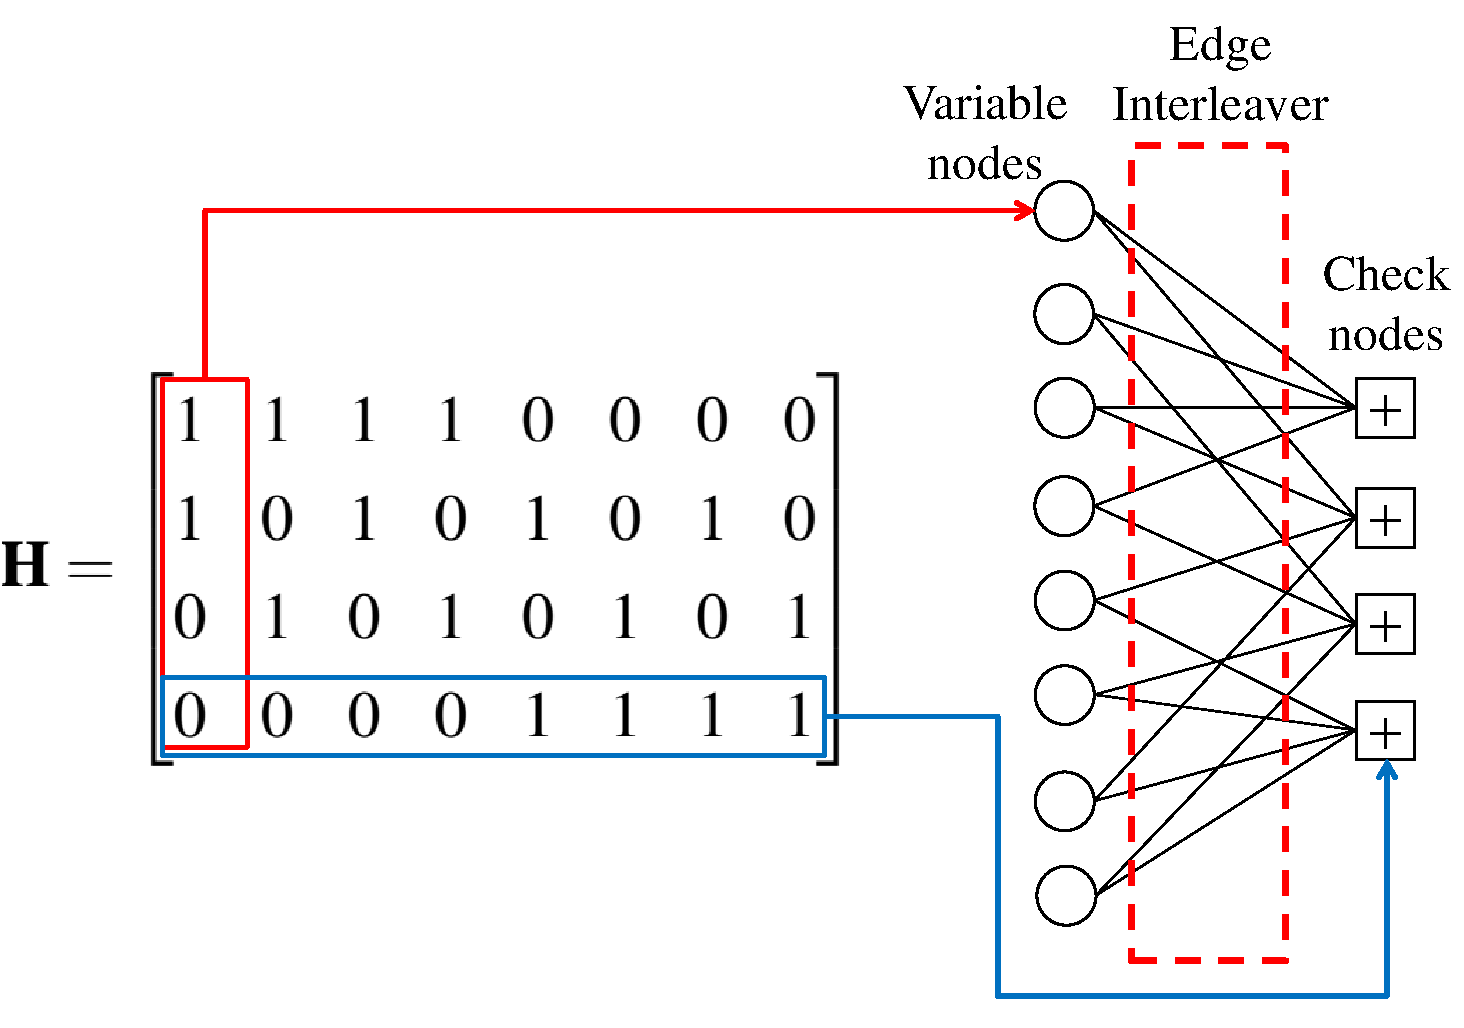
\includegraphics[scale=0.25]{pics/bipartitH1.pdf}
%\caption{Bipartite graph of parity check matrix $\mathbf{H}$.}
%\label{bipartitH} 
%\end{figure}
%\end{columns}
%\end{frame}
%\begin{frame}{Tanner Graph of The Proposed DVB-T2 LDPC Codes}
%%--------------------------
%\vspace{-0.5cm}
%	\begin{figure}
%		
%		\centering
%		
%		\begin{tikzpicture}[scale=0.5, transform shape]
%
%		
%		\draw (1,-6) -- (2.45,-6)[->];
%		\node at (2.45,-5.7) {$\hat{c}_{LDPC}$};
%		\node at (2.45,-6.4) {$L_{ch}$};
%
%		\draw (1,-6) -- (3.5,-6);
%		\draw (1,-7.5) -- (3.5,-7.5);
%		\draw (1,-7.5) -- (2.45,-7.5)[->];
%\node at (5.35,-6.25) {$L_{E_{v_{i}}}$};
%\node at (6.35,-6.8) {$L_{A_{c_{j}}}$};
%
%		\draw (1,-9) -- (3.5,-9);
%		\draw (1,-10.5) -- (3.5,-10.5);
%		\draw (1,-12.5) -- (3.5,-12.5);
%		\draw (1,-12.5) -- (2.45,-12.5)[->];
%	\node at (5.25,-12.85) {$L_{A_{ v_{i}}}$};
%\node at (6.45,-12.85) {$L_{E_{c_{j}}}$};
%
%		
%		
%		\draw (7,-8) rectangle (8,-7); \node at (7.5,-7.5) {$C_1$};
%		\draw (7,-8.5) rectangle (8,-9.5); \node at (7.5,-9) {$C_2$};
%		\draw (7,-10) rectangle (8,-11); \node at (7.5,-10.5) {$C_3$};
%		\draw (7.5,-11.3) [loosely dotted]-- (7.5,-11.7);
%		\draw (7,-12) rectangle (8,-13); \node at (7.5,-12.5) {$C_{9000}$};
%		
%		\draw (4,-6) circle [radius=0.5]; \node at (4,-6) {$V_{1}$};
%		\draw (4,-7.5) circle [radius=0.5]; \node at (4,-7.5) {$V_{2}$};
%		\draw (4,-9) circle [radius=0.5]; \node at (4,-9) {$V_{3}$};
%		\draw (4,-10.5) circle [radius=0.5]; \node at (4,-10.5) {$V_{4}$};
%		\draw (4,-11.3) [loosely dotted] -- (4,-11.7);
%		\draw (4,-12.5) circle [radius=0.5]; \node at (4,-12.5) {$V_{16200}$};
%		\draw (3.4,-5.3) [dashed] rectangle (4.6,-13.25);
%		\draw (4,-13.25) -- (4,-14.25);
%		\draw (4,-14.25) -- (9.5,-14.25) [->];
%		\draw (9.5,-10)  rectangle (13.5,-15); \node at (11.45,-12.5) {$BCH DECODER$};
%		\draw (13.5,-12.5) -- (15.85,-12.5) [->];\node at (14.55,-12.2) {$\hat{b}$}; 
%		\node at (8,-14) {$\hat{c}_{BCH}$};
%
%		
%		\draw (5.75,-6) [dotted]--  (5.75,-13);
%		\draw (5.75,-6) --  (6.25,-6)[->];
%		\node at (7.5,-6) {EXIT chart};
%		
%		
%		
%		\draw (4.5,-6) -- (7,-7.5);
%		\draw (4.5,-6) -- (5.75,-6.75)[->];
%		
%		\draw (4.5,-7.5) -- (7,-7.5);
%		\draw (4.5,-7.5) -- (7,-9);
%		\draw (4.5,-9) -- (7,-9);
%		\draw (4.5,-9) -- (7,-10.5);
%		\draw (4.5,-10.5) -- (7,-10.5);
%		\draw (4.5,-10.5) -- (7,-12.5);
%		\draw (4.5,-12.5) -- (7,-12.5);
%	
%		\draw (5.65,-12.5) -- (7,-12.5)[<-];
%		
%	\node at (12.55,-6.25) {\underline{Descriptions}};
%		\draw (9.25,-7.5) circle [radius=0.5]; \node at (9.25,-7.5) {$V$};
%		\node at (13.25,-7.5)  {: $V$ is variable nodes of LDPC};
%
%        \draw (8.75,-9.5) rectangle (9.75,-8.5); \node at (9.25,-9) {$C$};
%        \node at (13.05,-9) {: $C$ is check nodes of LDPC};
%
%        % \node at (13.55,-7.9) {: are degree distribution of EP VND};
%
%        % \node at (13.55,-8.6) {: are degree distribution of EP CND};
%		
%		
%		\end{tikzpicture}
%		\label{fig:tg}
%	\end{figure}
%	\vspace{-0.45cm}
%$L_{E_{v_{i}}}$ and $L_{E_{c_{j}}}$ are expressed\blfootnote{\tiny{S. ten Brink, “Convergence Behavior of Iteratively Decoded Parallel Concatenated Codes,” IEEE Transactions on Communications, vol. 49, no. 10, pp. 1727–1737, Oct 2001.}}
%\begin{columns}
%\column{.5\textwidth}
%\vspace{-0.2cm}
%\begin{equation}
%L_{E_{v_{i}}}(n)=L_{ch}+\sum_{j=1,j\neq i}^{d_{v_{n}}} L_{A_{v_j}},
%\end{equation}
%
%\column{.5\textwidth}
%\vspace{-0.1cm}
%\begin{equation}
%L_{E_{c_{j}}}(k)=\sum_{i=1,i\neq j}^{d_{c_{k}}}\boxplus L_{A_{c_{i}}}.
%\end{equation}
%
%
%\end{columns}
%
%\end{frame}




%=======================================================
%=======================================================
\section{The Design of DVB-T2 LDPC Codes}

\subsection{Proposed Downscaling Technique}
%--------------------------
%\begin{frame}{The Downscaled Technique for DVB-T2 LDPC Codes (1/2)}
%%--------------------------
%\vspace{-0.35cm}
%\begin{columns}
%\column{.45 \textwidth}
%\begin{table}[tb]
%\begin{adjustbox}{width=0.8\textwidth , totalheight=\textheight-2\baselineskip,keepaspectratio}
%	\begin{tabular}{|l|l|l|lllll}
%		\hline
%		\multicolumn{1}{|c|}{20} & \multicolumn{1}{c|}{712}  & \multicolumn{1}{c|}{2386} & \multicolumn{1}{c|}{6354} & \multicolumn{1}{c|}{4061} & \multicolumn{1}{c|}{1062} & \multicolumn{1}{c|}{5045} & \multicolumn{1}{c|}{5158} \\ \hline
%		\multicolumn{1}{|c|}{21} & \multicolumn{1}{c|}{2543} & \multicolumn{1}{c|}{5748} & \multicolumn{1}{c|}{4822} & \multicolumn{1}{c|}{2348} & \multicolumn{1}{c|}{3089} & \multicolumn{1}{c|}{6328} & \multicolumn{1}{c|}{5876} \\ \hline
%		\multicolumn{1}{|c|}{22} & \multicolumn{1}{c|}{926}  & \multicolumn{1}{c|}{5701} & \multicolumn{1}{c|}{269}  & \multicolumn{1}{c|}{3693} & \multicolumn{1}{c|}{2438} & \multicolumn{1}{c|}{3190} & \multicolumn{1}{c|}{3507} \\ \hline
%		\multicolumn{1}{|c|}{23} & \multicolumn{1}{c|}{2802} & \multicolumn{1}{c|}{4520} & \multicolumn{1}{c|}{3577} & \multicolumn{1}{c|}{5324} & \multicolumn{1}{c|}{1091} & \multicolumn{1}{c|}{4667} & \multicolumn{1}{c|}{4449} \\ \hline
%		\multicolumn{1}{|c|}{24} & \multicolumn{1}{c|}{5140} & \multicolumn{1}{c|}{2003} & \multicolumn{1}{c|}{1263} & \multicolumn{1}{c|}{4742} & \multicolumn{1}{c|}{6497} & \multicolumn{1}{c|}{1185} & \multicolumn{1}{c|}{6202} \\ \hline
%		0                        & 4046                      & 6934                      &                           &                           &                           &                           &                           \\ \cline{1-3}
%		1                        & 2855                      & 66                        &                           &                           &                           &                           &                           \\ \cline{1-3}
%		2                        & 6694                      & 212                       &                           &                           &                           &                           &                           \\ \cline{1-3}
%		3                        & 3439                      & 1158                      &                           &                           &                           &                           &                           \\ \cline{1-3}
%		4                        & 3850                      & 4422                      &                           &                           &                           &                           &                           \\ \cline{1-3}
%		5                        & 5924                      & 290                       &                           &                           &                           &                           &                           \\ \cline{1-3}
%		6                        & 1467                      & 4049                      &                           &                           &                           &                           &                           \\ \cline{1-3}
%		7                        & 7820                      & 2242                      &                           &                           &                           &                           &                           \\ \cline{1-3}
%		8                        & 4606                      & 3080                      &                           &                           &                           &                           &                           \\ \cline{1-3}
%		9                        & 4633                      & 7877                      &                           &                           &                           &                           &                           \\ \cline{1-3}
%		10                       & 3884                      & 6868                      &                           &                           &                           &                           &                           \\ \cline{1-3}
%		11                       & 8935                      & 4996                      &                           &                           &                           &                           &                           \\ \cline{1-3}
%		12                       & 3028                      & 764                       &                           &                           &                           &                           &                           \\ \cline{1-3}
%		13                       & 5988                      & 1057                      &                           &                           &                           &                           &                           \\ \cline{1-3}
%		14                       & 7411                      & 3450                      &                           &                           &                           &                           &                           \\ \cline{1-3}
%	\end{tabular}
%	            \end{adjustbox}
%
%\end{table}
%\column{.55 \textwidth}
%\begin{itemize}
%
%\item State the scaling factor $s_f$, where the factor must be divisors of $360$.  $360$ is the number of node indices of DVB-T2 LDPC codes.
%\item Fill $p_{1}(j), p_{2}(j), p_{3}(j), \dots, p_{q}(j), j= 1, 2, 3, \dots, J$  and $q= 1, 2, 3, \dots, Q$. 
%\item Calculate $r_{1}(j), r_{2}(j), r_{3}(j), \dots, r_{q}(j)$ \begin{flalign}
%r_{q}(j) = mod \{ \left [ p_q(j) + J\times \left ( k-1 \right ) \right ], \nonumber  \left [ P/s_f \right ] \} , 
%\end{flalign}
%\begin{flalign}
%1< k\leq \left ( 360/s_f \right ).
%\end{flalign}
%
%
%\item The new table of addresses parity bit accumulators $r_q$ are obtained.
%
%\end{itemize}
%%Where $q$ is amount of column and $j$ is amount of row from addresses of parity bit accumulators, $s_f$ is the scaling factor, $P$ is amount of $N-K$ in the original DVB-T2 LDPC codes, and the range of k is $1< k\leq \left ( 360/s_f \right )$. 
%\end{columns}
%\blfootnote{\tiny{F. A. Newagy and S. H. Elramly, “Novel Technique for Scaling Down LDPC Code Lengths in DVB-T2 Standard,” in 2012 International Conference on Telecommunications and Multimedia (TEMU), July 2012, pp. 180–184.}}
%\end{frame}

%--------------------------
\begin{frame}{Proposed (1): Downscaling Technique for DVB-T2 LDPC Codes }
%--------------------------
\begin{figure}
\centering 
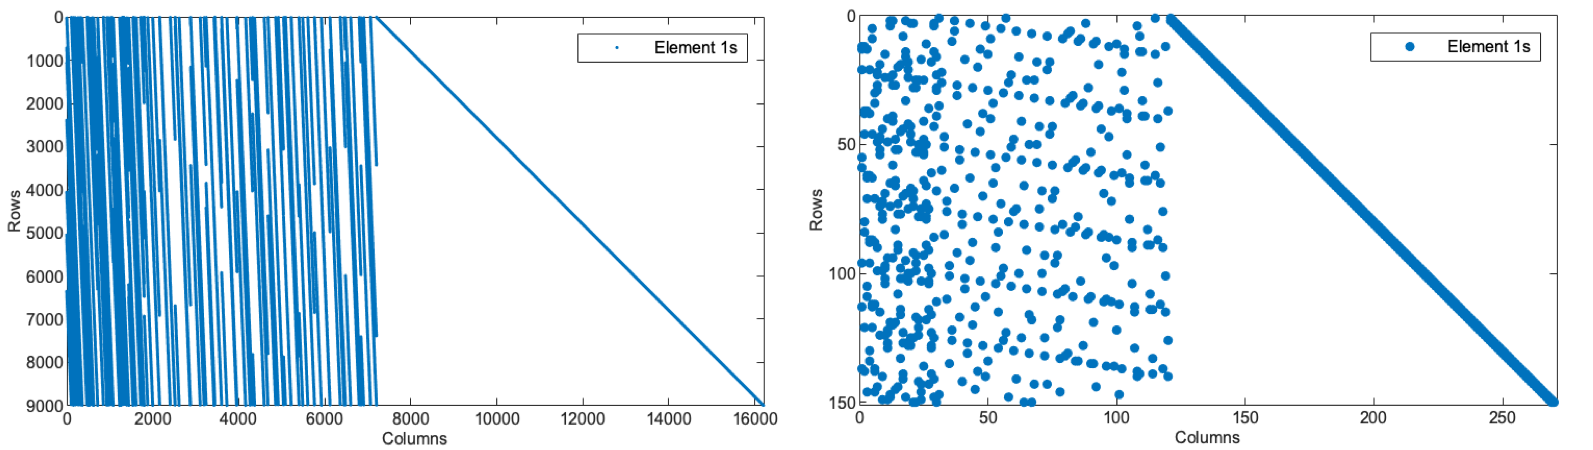
\includegraphics[scale=0.35]{gambarafa/compareH}

\label{sistemmodelMQCLDPC} %~\ref{kucing}
\end{figure}
%\begin{itemize}
%\item The comparison between parity check matrix of LDPC codes with a block length $N_{LDPC} = 16200$ and $N_{LDPC} = 270$.
%
%\item With $s_f=60$ and the DVB-T2 LDPC codes with block length $N_{LDPC}=16200$ is reduce to matrix LDPC codes $N_{LDPC}=270$, so the size of matrix will be smaller become .
%\end{itemize}

\begin{itemize}
	
	\item State the scaling factor $s_f$, where the factor must be divisors of $360$.  $360$ is the number of node indices of DVB-T2 LDPC codes.
	\item Fill $p_{1}(j), p_{2}(j), p_{3}(j), \dots, p_{q}(j), j= 1, 2, 3, \dots, J$  and $q= 1, 2, 3, \dots, Q$ with the value of addresses parity bit accumulator. 
	\item Calculate $r_{1}(j), r_{2}(j), r_{3}(j), \dots, r_{q}(j)$ \begin{flalign}
	r_{q}(j) = mod \{ \left [ p_q(j) + J\times \left ( k-1 \right ) \right ], \nonumber  \left [ P/s_f \right ] \} , 
	\end{flalign}
	\begin{flalign}
	1< k\leq \left ( 360/s_f \right ).
	\end{flalign}
	
	
	\item The new table of addresses parity bit accumulators $r_q$ are obtained.
	
\end{itemize}



%\begin{table}[tb]
%		\caption{addresses of parity bit accumulators for $N_{LDPC}=16200$ with code rate $R=\frac{1}{2}$.}
%	\label{table:accu}
%	\begin{tabular}{|l|l|l|lllll}
%		\hline
%		\multicolumn{1}{|c|}{20} & \multicolumn{1}{c|}{712}  & \multicolumn{1}{c|}{2386} & \multicolumn{1}{c|}{6354} & \multicolumn{1}{c|}{4061} & \multicolumn{1}{c|}{1062} & \multicolumn{1}{c|}{5045} & \multicolumn{1}{c|}{5158} \\ \hline
%		\multicolumn{1}{|c|}{21} & \multicolumn{1}{c|}{2543} & \multicolumn{1}{c|}{5748} & \multicolumn{1}{c|}{4822} & \multicolumn{1}{c|}{2348} & \multicolumn{1}{c|}{3089} & \multicolumn{1}{c|}{6328} & \multicolumn{1}{c|}{5876} \\ \hline
%		\multicolumn{1}{|c|}{22} & \multicolumn{1}{c|}{926}  & \multicolumn{1}{c|}{5701} & \multicolumn{1}{c|}{269}  & \multicolumn{1}{c|}{3693} & \multicolumn{1}{c|}{2438} & \multicolumn{1}{c|}{3190} & \multicolumn{1}{c|}{3507} \\ \hline
%		\multicolumn{1}{|c|}{23} & \multicolumn{1}{c|}{2802} & \multicolumn{1}{c|}{4520} & \multicolumn{1}{c|}{3577} & \multicolumn{1}{c|}{5324} & \multicolumn{1}{c|}{1091} & \multicolumn{1}{c|}{4667} & \multicolumn{1}{c|}{4449} \\ \hline
%		\multicolumn{1}{|c|}{24} & \multicolumn{1}{c|}{5140} & \multicolumn{1}{c|}{2003} & \multicolumn{1}{c|}{1263} & \multicolumn{1}{c|}{4742} & \multicolumn{1}{c|}{6497} & \multicolumn{1}{c|}{1185} & \multicolumn{1}{c|}{6202} \\ \hline
%		0                        & 4046                      & 6934                      &                           &                           &                           &                           &                           \\ \cline{1-3}
%		1                        & 2855                      & 66                        &                           &                           &                           &                           &                           \\ \cline{1-3}
%		2                        & 6694                      & 212                       &                           &                           &                           &                           &                           \\ \cline{1-3}
%		3                        & 3439                      & 1158                      &                           &                           &                           &                           &                           \\ \cline{1-3}
%		4                        & 3850                      & 4422                      &                           &                           &                           &                           &                           \\ \cline{1-3}
%		5                        & 5924                      & 290                       &                           &                           &                           &                           &                           \\ \cline{1-3}
%		6                        & 1467                      & 4049                      &                           &                           &                           &                           &                           \\ \cline{1-3}
%		7                        & 7820                      & 2242                      &                           &                           &                           &                           &                           \\ \cline{1-3}
%		8                        & 4606                      & 3080                      &                           &                           &                           &                           &                           \\ \cline{1-3}
%		9                        & 4633                      & 7877                      &                           &                           &                           &                           &                           \\ \cline{1-3}
%		10                       & 3884                      & 6868                      &                           &                           &                           &                           &                           \\ \cline{1-3}
%		11                       & 8935                      & 4996                      &                           &                           &                           &                           &                           \\ \cline{1-3}
%		12                       & 3028                      & 764                       &                           &                           &                           &                           &                           \\ \cline{1-3}
%		13                       & 5988                      & 1057                      &                           &                           &                           &                           &                           \\ \cline{1-3}
%		14                       & 7411                      & 3450                      &                           &                           &                           &                           &                           \\ \cline{1-3}
%	\end{tabular}
%\end{table}

\end{frame}


%=======================================================
\subsection{Possible Design with PEG}
%
%

	

\begin{frame}{Proposed (2): Progresive Edge-Growth (PEG) Algorithm \blfootnote{\tiny Xiao-Yu Hu, E. Eleftheriou and D. -. Arnold, "Progressive edge-growth Tanner graphs," GLOBECOM'01. IEEE Global Telecommunications Conference (Cat. No.01CH37270), San Antonio, TX, 2001, pp. 995-1001 vol.2.}}
	
	
	
	
	\vspace{-0.5cm}
	\begin{figure}
		\centering
		%	\hspace{ -in}
		\vspace{-0.25cm}
				\hspace{ -1in}
	
		
		\begin{minipage}{.5\linewidth}
			\hspace{1cm}
			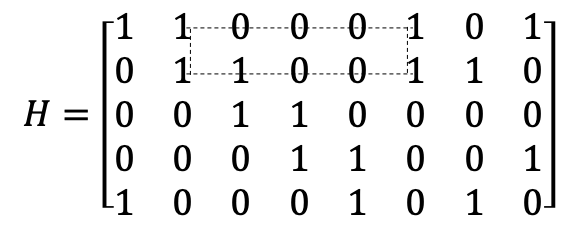
\includegraphics[width=2in]{PEG/girthhm}
			\vspace{-0.5cm}
			
			%		\center (a)
		\end{minipage}
		\hfill 	
		\hspace{ -1in}
		\begin{minipage}{.5\linewidth}
			\hspace{1cm}
			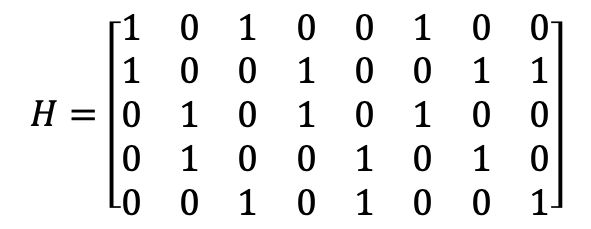
\includegraphics[width=2in]{PEG/peghm}
			
			\vspace{-0.5cm}
			%		\center (b)
		\end{minipage}
		\hfill
					\vspace{.255cm}
			\begin{minipage}{.5\linewidth}
			\hspace{3.5cm}
			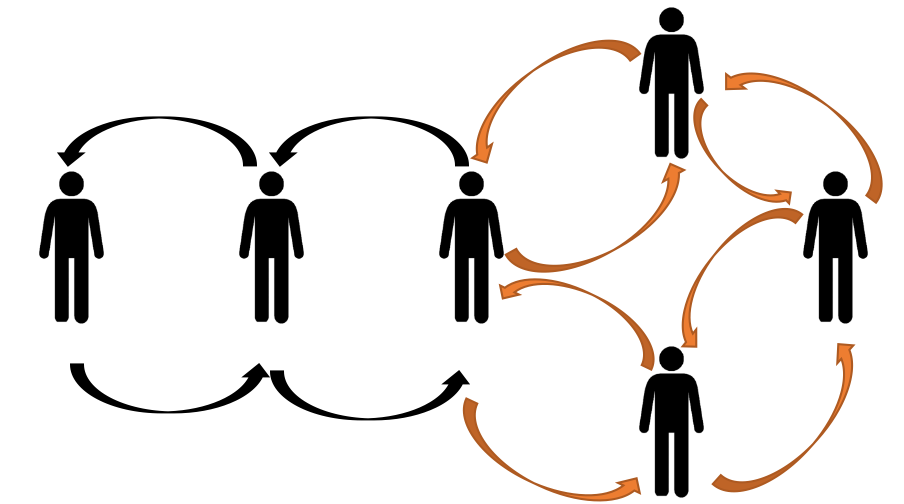
\includegraphics[width=1.25in]{gambarafa/lingkaransetan}
			\vspace{-1.55cm}
			
			%		\center (a)
		\end{minipage}
			\hspace{ -1in}
		\begin{minipage}{.5\linewidth}
		\hspace{2.5cm}
		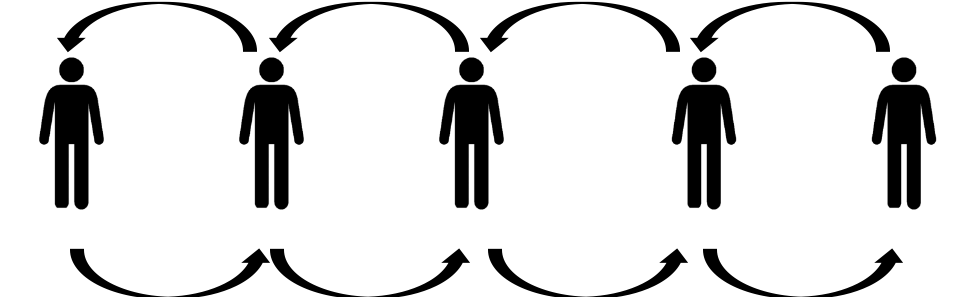
\includegraphics[width=1.25in]{gambarafa/soldier}
		\vspace{-1.95cm}
		
		%		\center (a)
	\end{minipage}
	
	
		%	\begin{minipage}{.5\linewidth}
		%		\hspace{-0.5cm}
		%		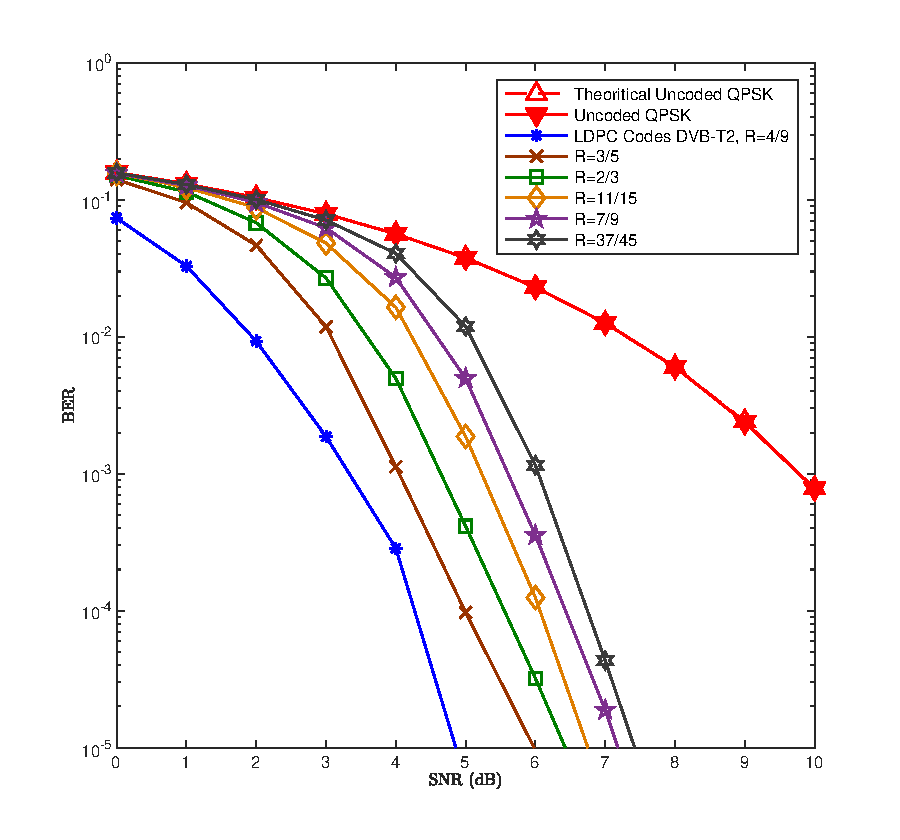
\includegraphics[width=3in]{hasilpegawgnfix.pdf}
		%		\vspace{-1.5cm}
		%		\center (c)
		%	\end{minipage}
		%	\hspace{-0.1 in}
		%	\begin{minipage}{.5\linewidth}
		%		%		\hspace{2.25 cm}
		%		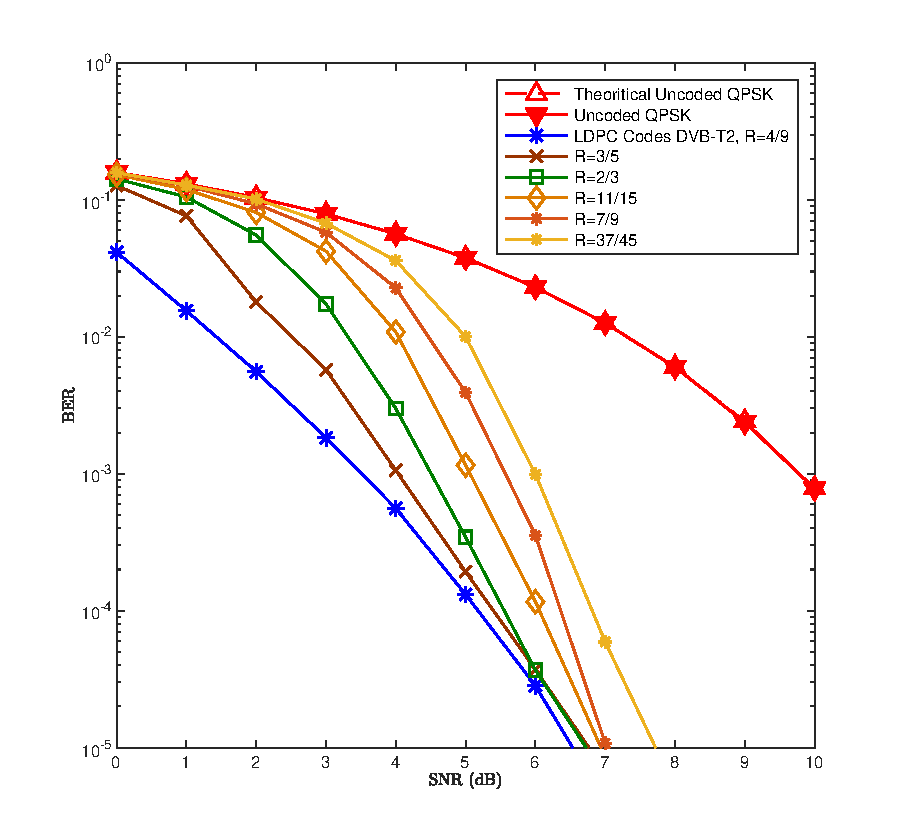
\includegraphics[width=3in]{hasilpegawgnfixLDGM.pdf}
		%		\vspace{-1.5cm}
		%		\center \hspace*{0.75cm}(d)
		%	\end{minipage}
		%	\caption {Kinerja BER LDPC \textit{codes} DVB-T2 dengan: (a) $N_{LDPC}=270$ menggunakan metode \textit{downscaled}, (b) $N_{LDPC}=16200$, (c) $N_{LDPC}=270$ menggunakan PEG dengan IRA, dan (d) $N_{LDPC}=270$ menggunakan PEG dengan LDGM pada kanal AWGN .}
		\label{gambar: ofdmhasil1}
	\end{figure}
	
	\vspace{1.15cm}
	%--------------------------
			\footnotesize
	\begin{itemize}

		\item Girth is the shortest cycle of LDPC codes that affect the LDPC codes performances, small girth will leave a bad effect on the LDPC codes decoders.\blfootnote{\tiny M. Sipser and D. A. Spielman, "Expander codes," in IEEE Transactions on Information Theory, vol. 42, no. 6, pp. 1710-1722, Nov. 1996.} 
		\item PEG is one of the method for constructing Tanner graphs having a large girth in a best-effort sense by progressively establishing edges between symbol and check nodes in an edge-by-edge manner.
		\item The proposed PEG Algortihm use the second method of PEG and use proposed algorithm to avoid girth-4 in LDPC codes.
		
%		\begin{equation}
%		H= \begin{bmatrix} 
%		1 & 1 & 0 & 0 & 0 & 1 & 0 & 1 \\ 
%		0 & 1 & 1 & 0 & 0 & 1 & 1 & 0  \\ 
%		0 & 0 & 1 & 1 & 0 & 0 & 0 & 0  \\ 
%		0 & 0 & 0 & 1 & 1 & 0 & 0 & 1    \\
%		1 & 0 & 0 & 0 & 1 & 0 & 1 & 0
%		\end{bmatrix} \;
%			H= \begin{bmatrix} 
%		1 & 0 & 1 & 0 & 0 & 1 & 0 & 0 \\ 
%		1 & 0 & 0 & 1 & 0 & 0 & 1 & 1  \\ 
%		0 & 1 & 0 & 1 & 0 & 1 & 0 & 0  \\ 
%		0 & 1 & 0 & 0 & 1 & 0 & 1 & 0    \\
%		0 & 0 & 1 & 0 & 1 & 0 & 0 & 1
%		\end{bmatrix}.
%		\label{eq: IRA}
%		\end{equation} 
		
		
%			\item Actually, PEG has two methods for constructing LDPC codes, there are:
%		\begin{enumerate}
%			\item to randomly select one of these check nodes.
%			\item to always select one according to its position in the order of  $c_1, c_2, c_3, \cdots, c_{m}$, with $m$ is amount of the rows.
%		\end{enumerate}
		
%		\item LDPC \textit{codes} construction step using PEG algorithm as follows
%		\begin{enumerate}
%			\item Places element 1 from first column until column $n^{th}$, this placement consider the row or check node with the lowest degree. 
%			\item Progressively establishing edges between symbol and check nodes in an edge-by-edge manner.
%		\end{enumerate}
%		\item Using PEG algorithm, LDPC codes can be constructed with based on known value of block length $n$, check node, degree distribution of each variable node and check node.
		\end{itemize} 
	
\end{frame}
%
%\begin{frame}{Progresive Edge-Growth (PEG) Algorithm (2/3) \blfootnote{\tiny Xiao-Yu Hu, E. Eleftheriou and D. -. Arnold, "Progressive edge-growth Tanner graphs," GLOBECOM'01. IEEE Global Telecommunications Conference (Cat. No.01CH37270), San Antonio, TX, 2001, pp. 995-1001 vol.2.}}
%
%
%\begin{columns}
%	\column{.5\textwidth}
%	\vspace{-1cm}
%	\begin{figure}
%		\centering 
%		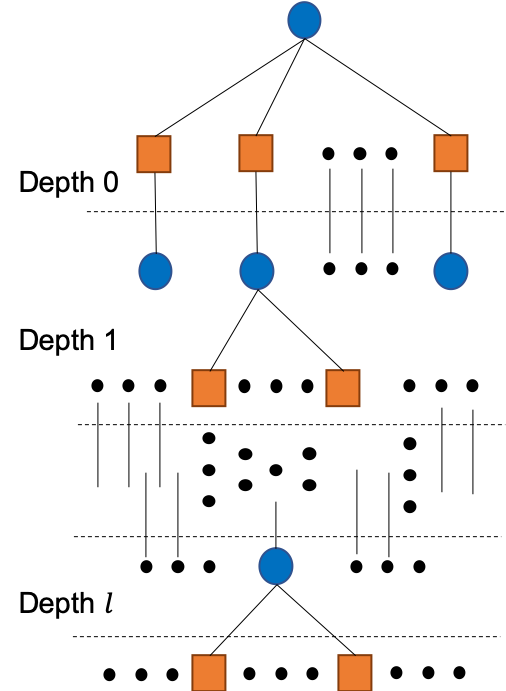
\includegraphics[scale=0.50]{PEG/contPEG}
%		\centering 
%	\end{figure}
%	\column{.5\textwidth}
%	\footnotesize {
%		\begin{itemize}
%			\item PEG algorithm construction is based on tree graph, tree graph constructed for each variable node.  The construction of PEG's tree graph has one condition to fulfill there is each node can be called once in the one tree graph.
%			\item From the constructed tree graph we can know depth $l$ from each tree graph, so girth bound from  constructed LDPC codes using PEG can be known from this equation 
%			\begin{equation}
%			t=\frac{\log\left ( md_c^{max}- \frac{md_c^{max}}{d_v^{max}} - m +1 \right )}{\log\left [ \left ( d_v^{max} -1  \right ) \left ( d_c^{max} -1  \right ) \right ]}-1,
%			\label{eq:t}
%			\end{equation}
%			\begin{equation}
%			g \geq 2 \left (\left \lfloor t \right \rfloor +2 \right ).
%			\label{eq:g}
%			\end{equation}
%%			dengan nilai $d_v$, $d_c$, dan $m$ yang telah ditentukan. Dari persamaan (\ref{eq:t}) dan (\ref{eq:g}) maka
%%			\begin{equation}
%%			\frac{d_v^{max}\left [  \left ( d_v^{max}-1 \right )^{t+1} \left ( d_c^{max}-1 \right )^{t+1} -1\right ]}{\left ( d_v^{max}-1 \right ) \left ( d_c^{max}-1 \right )-1}<m,
%%			\end{equation}
%%			sehingga dapat diketahui batas minimal jumlah \textit{check node} agar \textit{girth} yang ingin dihindari dapat terpenuhi.
%			
%		\end{itemize}
%		
%%		\begin{enumerate}
%%			\item State one variable node and progressively establishing edges between check and symbol nodes from the parity check matrix of LDPC codes.
%%			\item Keep spreading the edges for each node until find one node that can't spread the edges anymore.
%%			%			\item Tentukan satu \textit{variable node} dan sebarkan \textit{edges}-nya sesuai dari matriks.
%%			%			\item Sebarkan \textit{edges} terus menerus sampai terdapat \textit{node} yang tidak dapat menyebarkan \textit{edge}.
%%			\item Calculate the branch $b$ start from one, then with this equation
%%			\begin{equation}
%%			g=b\times 2,
%%			\end{equation}
%%			the local girth $g$ can be calculated.
%%			%			 nilai \textit{local girth} dapat diketahui.
%%	\end{enumerate} 
%}
%\end{columns}
% \end{frame}
%
%
%
%\begin{frame}{Progresive Edge-Growth (PEG) Algorithm (3/3) \blfootnote{\tiny Xiao-Yu Hu, E. Eleftheriou and D. -. Arnold, "Progressive edge-growth Tanner graphs," GLOBECOM'01. IEEE Global Telecommunications Conference (Cat. No.01CH37270), San Antonio, TX, 2001, pp. 995-1001 vol.2.}}
%	%--------------------------
%	\begin{itemize}
%		\footnotesize{
%		\item From these equation (\ref{eq:t}) and (\ref{eq:g}), it become
%		\begin{equation}
%		\frac{d_v^{max}\left [  \left ( d_v^{max}-1 \right )^{t+1} \left ( d_c^{max}-1 \right )^{t+1} -1\right ]}{\left ( d_v^{max}-1 \right ) \left ( d_c^{max}-1 \right )-1}<m,
%		\end{equation}
%		so, the desired LDPC codes can be constructed using this bound.
%		
%		\item Actually, PEG has two methods for constructing LDPC codes, there are:
%	\begin{enumerate}
%		\item to randomly select one of these check nodes.
%		\item to always select one according to its position in the order of  $c_1, c_2, c_3, \cdots, c_{m}$, with $m$ is amount of the rows.
%	\end{enumerate}
%	The first proposed PEG algorithm use first method. so, the proposed PEG algorithm in this thesis use the second method.\blfootnote{\tiny Xiao-Yu Hu, E. Eleftheriou and D. M. Arnold, "Regular and irregular progressive edge-growth tanner graphs," in IEEE Transactions on Information Theory, vol. 51, no. 1, pp. 386-398, Jan. 2005.}, sedangkan pada penelitian ini mengusulkan dengan menggunakan metode kedua.}
%\end{itemize}
%	
%\end{frame}
%
%
%%--------------------------
%%\begin{frame}{Progresive Edge-Growth (PEG) Algorithm (1/4)\footnote[1]{\tiny Xiao-Yu Hu, E. Eleftheriou and D. -. Arnold, "Progressive edge-growth Tanner graphs," GLOBECOM'01. IEEE Global Telecommunications Conference (Cat. No.01CH37270), San Antonio, TX, 2001, pp. 995-1001 vol.2.}}
%%	%--------------------------
%%	\begin{itemize}
%%		\item PEG adalah salah satu metode untuk membuat LDPC \textit{codes} berdasarkan dari Tanner \textit{graph} dengan memperhatikan penyebaran \textit{edge} yang terhubung pada setiap \textit{node} untuk menghasilkan \textit{girth} besar.
%%		\item Pembuatan LDPC codes dengan menggunakan PEG dapat dibuat berdasarkan jumlah \textit{variable nodes} atau \textit{block length} $n$, check node $m$, \textit{variable node degree} (VND), dan \textit{check node degree} (CND).
%%		\item PEG melakukan penyebaran \textit{edge} menggunakan graf pohon dengan memperhatikan \textit{degree} setiap \textit{node} yang telah ditentukan dan setiap \textit{node}-nya hanya dapat muncul sekali.
%%		\item Kedalaman dari graf pohon akan disimbolkan dengan $l$. $l$ akan mempengaruhi lokal \textit{girth} yang terbentuk.
%%	\end{itemize}
%%	
%%\end{frame}
%%
%%
%%%=======================================================
%%\begin{frame}{Progresive Edge-Growth (PEG) Algorithm (2/4)}
%%	%--------------------------
%%	Secara sederhana proses pembuatan LDPC \textit{codes} menggunakan algoritma PEG adalah sebagai  berikut:
%%	\begin{enumerate}
%%		\item Tempatkan elemen 1 mulai dari kolom ke-1 sampai ke-$n$, penempatan ini memperhatikan baris atau \textit{check node} dengan \textit{degree} terkecil.
%%		\item Menyebarkan \textit{edge} ke node yang belum terhubung dengan memperhatikan \textit{degree} dari \textit{check node}.
%%	\end{enumerate}
%%	\textit{Cycle} dari LDPC \textit{codes} yang terbentuk menggunakan PEG dapat dipastikan akan memenuhi 
%%	\begin{equation}
%%	2(l+2).
%%	\end{equation}
%%	
%%	
%%	
%%	
%%	%\blfootnote{\tiny{ETSI, Digital Video Broadcasting (DVB); Frame Structure Channel Coding and Modulation for a Second Generation Digital Terrestrial Television Broadcasting System (DVB-T2), 1st ed., ETSI, July 2015.}}
%%	%\begin{figure}
%%	%\centering
%%	%\hspace{-0.2in} 
%%	%\begin{tabular}{cl}
%%	%$\mathbf{H}=$ & \begin{tabular}[c]{@{}l@{}}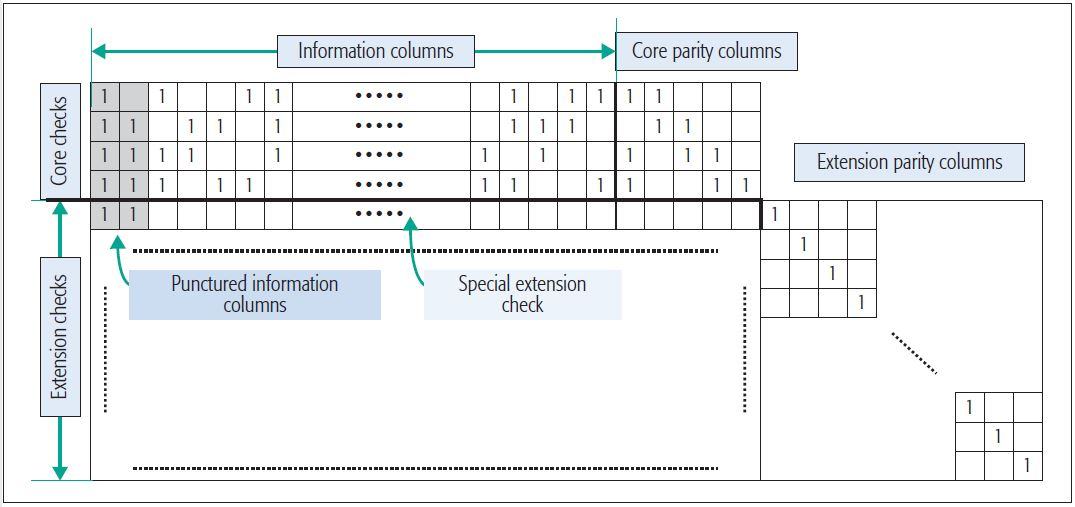
\includegraphics[scale=0.38]{pics/matriks5g}\end{tabular}
%%	%\end{tabular}
%%	%\caption{Sketch of base parity check structure for the 5G-NR LDPC codes \footnote{\tiny{T. Richardson and S. Kudekar, “Design of low-density parity check codes for 5G new radio,” IEEE Communications Magazine, vol. 56, no. 3, pp. 28–34, March 2018.}}.}
%%	%\label{5gsketch}
%%	%\end{figure}
%%	%\end{columns}
%%\end{frame}
%%%=======================================================
%%\begin{frame}{Progresive Edge-Growth (PEG) Algorithm (3/4)\footnote[1]{\tiny Xiao-Yu Hu, E. Eleftheriou and D. M. Arnold, "Regular and irregular progressive edge-growth tanner graphs," in IEEE Transactions on Information Theory, vol. 51, no. 1, pp. 386-398, Jan. 2005.
%%	}}
%%	%--------------------------
%%	%	Dalam perancangan LDPC \textit{codes} menggunakan algoritma PEG dengan nilai $d_v$, $d_c$, dan $m$ yang telah ditentukan, dapat diketahui batas dari nilai \textit{girth} melalui persamaan
%%	\vspace{-0.2cm}
%%	Batas nilai \textit{girth} $(g)$ pada LDPC \textit{codes} yang dirancang menggunakan algoritma PEG dapat diketahui melalui persamaan 
%%	\begin{equation}
%%	t=\frac{\log\left ( md_c^{max}- \frac{md_c^{max}}{d_v^{max}} - m +1 \right )}{\log\left [ \left ( d_v^{max} -1  \right ) \left ( d_c^{max} -1  \right ) \right ]}-1,
%%	\label{eq:t}
%%	\end{equation}
%%	\begin{equation}
%%	g \geq 2 \left (\left \lfloor t \right \rfloor +2 \right ),
%%	\label{eq:g}
%%	\end{equation}
%%	dengan nilai $d_v$, $d_c$, dan $m$ yang telah ditentukan. Dari persamaan (\ref{eq:t}) dan (\ref{eq:g}) maka
%%	\begin{equation}
%%	\frac{d_v^{max}\left [  \left ( d_v^{max}-1 \right )^{t+1} \left ( d_c^{max}-1 \right )^{t+1} -1\right ]}{\left ( d_v^{max}-1 \right ) \left ( d_c^{max}-1 \right )-1}<m,
%%	\end{equation}
%%	sehingga dapat diketahui batas minimal jumlah \textit{check node} agar \textit{girth} yang ingin dihindari dapat terpenuhi.
%%\end{frame}
%%
%%
%%
%%\begin{frame}{Progresive Edge-Growth (PEG) Algorithm (4/4)}
%%	%--------------------------
%%	PEG memiliki dua metode dalam proses pembuatan LDPC \textit{codes} dengan cara:
%%	\begin{enumerate}
%%		\item Secara acak memilih \textit{check nodes} terkecil yang ditemukan.
%%		\item Selalu memilih \textit{check nodes} terkecil yang ditemukan sesuai dengan urutannya $c_1, c_2, c_3, \cdots, c_{m}$, dengan $m$ adalah jumlah baris.
%%	\end{enumerate}
%%	Hal ini mengakibatkan LDPC \textit{codes} akan memiliki matriks \textit{parity check} berbeda-beda, apabila menggunakan algoritma PEG. Pada awalnya PEG menggunakan metode pertama\footnote[1]{\tiny Xiao-Yu Hu, E. Eleftheriou and D. M. Arnold, "Regular and irregular progressive edge-growth tanner graphs," in IEEE Transactions on Information Theory, vol. 51, no. 1, pp. 386-398, Jan. 2005.}, sedangkan pada penelitian ini mengusulkan dengan menggunakan metode kedua.
%%	
%%\end{frame}
%
%
%%\section{The Proposed PEG Algorithm for LDPC Codes }
%%--------------------------
%\begin{frame}{The Proposed PEG Algorithm for LDPC Codes (1/5)}
%	%--------------------------
%	\begin{itemize}
%		\item The proposed PEG Algortihm use the second method of PEG and using an proposed algorithm to avoid girth-4 in LDPC \textit{codes}.
%		\item The proposed Anti Girth-4 algorithm take place in the second step of PEG construction. This thesis summarize the proposed algorithm as follows:
%		\begin{figure}
%			\centering 
%			\includegraphics[scale=0.5]{PEG/step1}
%			\centering 
%		\end{figure}
%		\begin{itemize}
%			\item[1.] Create zeros matrix with dimension $m \times n$, with $n$ is the amount of variable nodes and $m$ is the amount of check nodes.
%%			Buat matriks nol dengan dimensi $m\times n$, dengan $n$ adalah jumlah variable \textit{nodes} dan $m$ adalah jumlah \textit{check nodes} yang telah ditentukan.
%		\end{itemize}
%
%	\end{itemize}
%	\blfootnote{\tiny{F. A. Newagy and S. H. Elramly, “Novel Technique for Scaling Down LDPC Code Lengths in DVB-T2 Standard,” in 2012 International Conference on Telecommunications and Multimedia (TEMU), July 2012, pp. 180–184.}}
%\end{frame}
%
%
%\begin{frame}{The Proposed PEG Algorithm for LDPC Codes (2/5)}
%	%--------------------------
%	
%	\centering 
%	\begin{figure}
%		\centering 
%		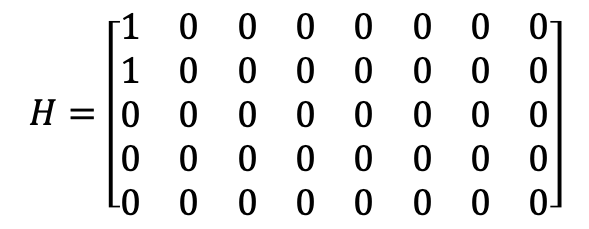
\includegraphics[scale=0.5]{PEG/step2}
%		\centering 
%	\end{figure}
%	\begin{itemize}
%		\item[2.] The first element 1 is placed from the first step of PEG algorithm process. The second element 1 until as much of $d_v(n)$ use the combination of PEG with Anti Girth-4 algorithm.  
%%		Elemen 1 pertama ditempatkan sesuai dengan algoritma pertama dari proses PEG. Elemen 1 kedua dan seterusnya sebanyak $d_v(n)$ ditempatkan menggunakan kombinasi algoritma PEG dengan \textit{Anti Girth}-4.
%	\end{itemize}
%	\centering 
%	\begin{figure}
%		\centering 
%		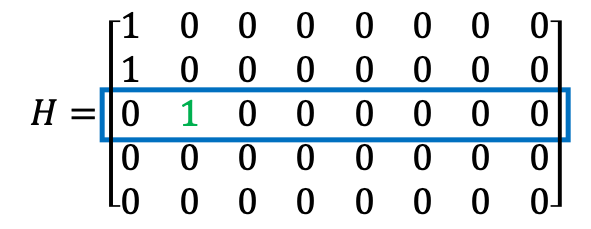
\includegraphics[scale=0.5]{PEG/step3}
%		\centering 
%	\end{figure}
%	\begin{itemize}
%		\item[3.] Element 1 placed on the first check node with the lowest degree.
%	\end{itemize}
%\end{frame}
%
%
%\begin{frame}{The Proposed PEG Algorithm for LDPC Codes (3/5)}
%	%--------------------------
%	
%	\centering 
%	\begin{figure}
%		\centering 
%		
\includegraphics[scale=0.5]{PEG/step4}
%		\centering 
%	\end{figure}
%	\begin{itemize}
%		\item[4.] Symbol $x$ is the candidate for element 1 position, $x$ is choosed because $x$'s row is row with the lowest degree. For the next step, this algorithm use proposed the Anti Girth 4 algorithm by checking from left to the right until $x$'s position. When there are no element 1, it can be assured that $x$ will not form girth 4.
%		
%	\end{itemize}
%	
%\end{frame}
%
%
%\begin{frame}{The Proposed PEG Algorithm for LDPC Codes (4/5)}
%	
%	\centering 
%	\begin{figure}
%		\centering 
%		\hspace{2cm}
%		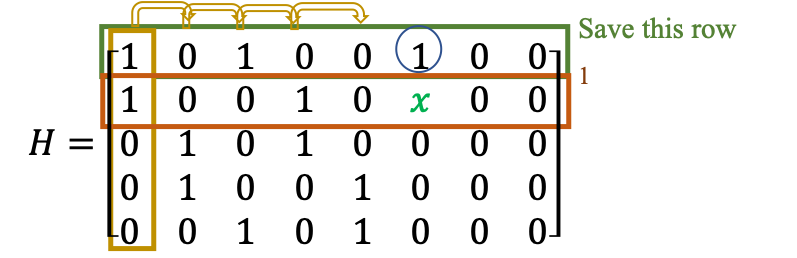
\includegraphics[scale=0.5]{PEG/step5eng}
%		\centering 
%	\end{figure}
%	\begin{itemize}
%		
%		\item[5.] The first step of Anti Girth 4 algorithm start with saving the row from the previous element one in $x$'s column. Then do the checking process of element 1 from left to the right until $x$'s position, if the checking process found element 1, the algorithm will do the next step. If there are no element 1 in this checking process, $x$ will be element 1.
%%		\item[5.] Algoritma \textit{Anti Girth}-4 dimulai dari iterasi ke-1, baris dari elemen 1 sebelumnya disimpan yang nantinya akan digunakan pada pengecekan akhir. Kemudian melakukan pengecekan dari kiri ke kanan apabila ditemukan elemen 1, maka akan berlanjut ke iterasi berikutnya. Apabila tidak ditemukan elemen 1 pada kolom tersebut, maka $x$ akan menjadi elemen 1. Pengecekan akan dilakukan sampai kolom sebelum kolom dari $x$.
%	\end{itemize}
%	
%	
%	
%	
%	
%\end{frame}
%
%
%
%
%\begin{frame}{The Proposed PEG Algorithm for LDPC Codes (5/5)}
%	
%	\centering 
%	\begin{figure}
%		\centering 
%		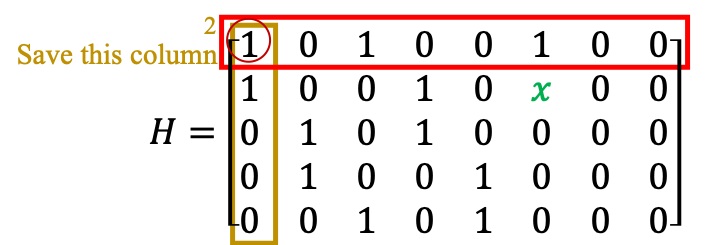
\includegraphics[scale=0.5]{PEG/step6eng}
%		\centering 
%	\end{figure}
%	\begin{itemize}
%		\item[6.] The second step of Anti Girth 4 start with saving the  column from element 1 that has been found in the first step.
%		\item [7.] Then do the final checking, if only if
%		\begin{equation}
%		H_{Saved\_row, Saved\_column}=1,
%		\end{equation}
%		$x$ will move to the next row with the lowest degree, because if $x$ become element 1 the girth 4 will be formed.
%%		if $x$ is element 1 the girth 4 will be formed, so $x$ will move to the next row with the lowest degree.
%%		\item [7.] Kemudian melakukan pengecekan akhir, yaitu apabila
%%		\begin{equation}
%%		H_{Baris\_simpan, Kolom\_simpan}=1,
%%		\end{equation}
%%		pada $x$ akan terbentuk \textit{girth} 4 jika $x$ berelemen 1, sehingga $x$ akan berpindah ke \textit{check node} dengan CND minimal berikutnya dan melakukan pengecekan lagi.
%	\end{itemize}
%\end{frame}
%
%
%%--------------------------
%%\begin{frame}{The Proposed Anti Girth-4 Algorithm (1/5)}
%%	%--------------------------
%%	
%%	\centering 
%%	\begin{itemize}
%%		\item Algoritma anti \textit{girth}-4 ini ditambahkan pada iterasi kedua dalam penempatan elemen satu di setiap kolom. Langkah-langkah perancangan matriks dan pengecekannya sebagai berikut:
%%		\begin{figure}
%%			\centering 
%%			\includegraphics[scale=0.5]{PEG/step1}
%%			\centering 
%%		\end{figure}
%%		\begin{itemize}
%%			\item[1.] Buat matriks nol dengan dimensi $m\times n$, dengan $n$ adalah jumlah variable \textit{nodes} dan $m$ adalah jumlah \textit{check nodes} yang telah ditentukan.
%%		\end{itemize}
%%		%\begin{enumerate}
%%		%	\begin{figure}
%%		%			\centering 
%%		%		\includegraphics[scale=0.5]{gambarafa/step1}
%%		%		\centering 
%%		%	\end{figure}
%%		%	\item Melukakan pencarian elemen 1 pada kolom yang sama dengan posisi yang akan kita tambahkan elemen 1, apabila ditemukan simpan baris dari elemen 1 tersebut.
%%		%	\item Kemudian melakukan pengecekan kembali pada satu baris yang sama dengan posisi yang akan kita tambahkan elemen 1, apabila ditemukan simpan kolom dari elemen satu tersebut.
%%		%	\item Apabila pada langkah pertama dan kedua tidak ditemukan elemen satu maka posisi yang akan kita tambahkan elemen 1 akan aman dari \textit{girth}-4, jika ditemukan maka lanjut ke langkah berikutnya.
%%		%	\item Melakukan pengecekan pada elemen matriks dengan kolom dan baris yang tersimpan, apabila bernilai 1 maka posisi tersebut tidak boleh bernilai 1 jika tidak maka posisi tersebut dapat bernilai 1.
%%		%\end{enumerate}
%%		
%%	\end{itemize}
%%	
%%	
%%	
%%	
%%	
%%	%\begin{table}[tb]
%%	%		\caption{addresses of parity bit accumulators for $N_{LDPC}=16200$ with code rate $R=\frac{1}{2}$.}
%%	%	\label{table:accu}
%%	%	\begin{tabular}{|l|l|l|lllll}
%%	%		\hline
%%	%		\multicolumn{1}{|c|}{20} & \multicolumn{1}{c|}{712}  & \multicolumn{1}{c|}{2386} & \multicolumn{1}{c|}{6354} & \multicolumn{1}{c|}{4061} & \multicolumn{1}{c|}{1062} & \multicolumn{1}{c|}{5045} & \multicolumn{1}{c|}{5158} \\ \hline
%%	%		\multicolumn{1}{|c|}{21} & \multicolumn{1}{c|}{2543} & \multicolumn{1}{c|}{5748} & \multicolumn{1}{c|}{4822} & \multicolumn{1}{c|}{2348} & \multicolumn{1}{c|}{3089} & \multicolumn{1}{c|}{6328} & \multicolumn{1}{c|}{5876} \\ \hline
%%	%		\multicolumn{1}{|c|}{22} & \multicolumn{1}{c|}{926}  & \multicolumn{1}{c|}{5701} & \multicolumn{1}{c|}{269}  & \multicolumn{1}{c|}{3693} & \multicolumn{1}{c|}{2438} & \multicolumn{1}{c|}{3190} & \multicolumn{1}{c|}{3507} \\ \hline
%%	%		\multicolumn{1}{|c|}{23} & \multicolumn{1}{c|}{2802} & \multicolumn{1}{c|}{4520} & \multicolumn{1}{c|}{3577} & \multicolumn{1}{c|}{5324} & \multicolumn{1}{c|}{1091} & \multicolumn{1}{c|}{4667} & \multicolumn{1}{c|}{4449} \\ \hline
%%	%		\multicolumn{1}{|c|}{24} & \multicolumn{1}{c|}{5140} & \multicolumn{1}{c|}{2003} & \multicolumn{1}{c|}{1263} & \multicolumn{1}{c|}{4742} & \multicolumn{1}{c|}{6497} & \multicolumn{1}{c|}{1185} & \multicolumn{1}{c|}{6202} \\ \hline
%%	%		0                        & 4046                      & 6934                      &                           &                           &                           &                           &                           \\ \cline{1-3}
%%	%		1                        & 2855                      & 66                        &                           &                           &                           &                           &                           \\ \cline{1-3}
%%	%		2                        & 6694                      & 212                       &                           &                           &                           &                           &                           \\ \cline{1-3}
%%	%		3                        & 3439                      & 1158                      &                           &                           &                           &                           &                           \\ \cline{1-3}
%%	%		4                        & 3850                      & 4422                      &                           &                           &                           &                           &                           \\ \cline{1-3}
%%	%		5                        & 5924                      & 290                       &                           &                           &                           &                           &                           \\ \cline{1-3}
%%	%		6                        & 1467                      & 4049                      &                           &                           &                           &                           &                           \\ \cline{1-3}
%%	%		7                        & 7820                      & 2242                      &                           &                           &                           &                           &                           \\ \cline{1-3}
%%	%		8                        & 4606                      & 3080                      &                           &                           &                           &                           &                           \\ \cline{1-3}
%%	%		9                        & 4633                      & 7877                      &                           &                           &                           &                           &                           \\ \cline{1-3}
%%	%		10                       & 3884                      & 6868                      &                           &                           &                           &                           &                           \\ \cline{1-3}
%%	%		11                       & 8935                      & 4996                      &                           &                           &                           &                           &                           \\ \cline{1-3}
%%	%		12                       & 3028                      & 764                       &                           &                           &                           &                           &                           \\ \cline{1-3}
%%	%		13                       & 5988                      & 1057                      &                           &                           &                           &                           &                           \\ \cline{1-3}
%%	%		14                       & 7411                      & 3450                      &                           &                           &                           &                           &                           \\ \cline{1-3}
%%	%	\end{tabular}
%%	%\end{table}
%%	
%%\end{frame}
%%
%%
%%\begin{frame}{The Proposed Anti Girth-4 Algorithm (2/5)}
%%	%--------------------------
%%	
%%	\centering 
%%	\begin{figure}
%%		\centering 
%%		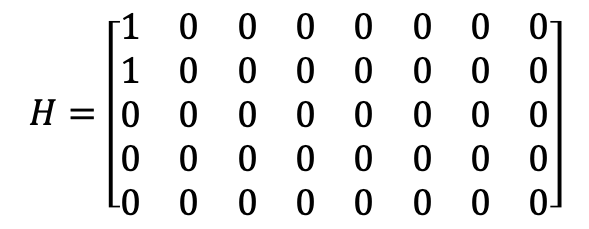
\includegraphics[scale=0.5]{PEG/step2}
%%		\centering 
%%	\end{figure}
%%	\begin{itemize}
%%		\item[2.] Elemen 1 pertama ditempatkan sesuai dengan algoritma pertama dari proses PEG. Elemen 1 kedua dan seterusnya sebanyak $d_v(n)$ ditempatkan menggunakan kombinasi algoritma PEG dengan \textit{Anti Girth}-4.
%%	\end{itemize}
%%	\centering 
%%	\begin{figure}
%%		\centering 
%%		\includegraphics[scale=0.5]{PEG/step3}
%%		\centering 
%%	\end{figure}
%%	\begin{itemize}
%%		\item[3.] Elemen 1 ditempatkan pada \textit{check node} urutan pertama dengan nilai CND terendah.
%%	\end{itemize}
%%\end{frame}
%%%=======================================================
%%\begin{frame}{The Proposed Anti Girth-4 Algorithm (3/5)}
%%	%--------------------------
%%	
%%	\centering 
%%	\begin{figure}
%%		\centering 
%%		\includegraphics[scale=0.75]{PEG/step4}
%%		\centering 
%%	\end{figure}
%%	\begin{itemize}
%%		\item[4.] Simbol $x$ adalah calon letak elemen 1, $x$ dipilih berdasarkan baris yang memiliki nilai CND terendah. Kemudian langkah berikutnya menggunakan algoritma \textit{Anti Girth}-4, melakukan pengeceken ke kiri apabila tidak ada elemen satu maka letak tersebut akan menjadi elemen 1.
%%	\end{itemize}
%%	
%%\end{frame}
%%
%%%--------------------------
%%\begin{frame}{The Proposed Anti Girth-4 Algorithm (4/5)}
%%	
%%	\centering 
%%	\begin{figure}
%%		\centering 
%%		\includegraphics[scale=0.65]{PEG/step5}
%%		\centering 
%%	\end{figure}
%%	\begin{itemize}
%%		\item[5.] Algoritma \textit{Anti Girth}-4 dimulai dari iterasi ke-1, baris dari elemen 1 sebelumnya disimpan yang nantinya akan digunakan pada pengecekan akhir. Kemudian melakukan pengecekan dari kiri ke kanan apabila ditemukan elemen 1, maka akan berlanjut ke iterasi berikutnya. Apabila tidak ditemukan elemen 1 pada kolom tersebut, maka $x$ akan menjadi elemen 1. Pengecekan akan dilakukan sampai kolom sebelum kolom dari $x$.
%%	\end{itemize}
%%	
%%	
%%	
%%	
%%	
%%\end{frame}
%%
%%\begin{frame}{The Proposed Anti Girth-4 Algorithm (5/5)}
%%	
%%	\centering 
%%	\begin{figure}
%%		\centering 
%%		\includegraphics[scale=0.65]{PEG/step6}
%%		\centering 
%%	\end{figure}
%%	\begin{itemize}
%%		\item[5.] Iterasi ke-2 Algoritma \textit{Anti Girth}-4, menyimpan kolom dari elemen 1 yang ditemukan pada proses pengecekan di iterasi ke-1. 
%%		\item [6.] Kemudian melakukan pengecekan akhir, yaitu apabila
%%		\begin{equation}
%%		H_{Baris\_simpan, Kolom\_simpan}=1,
%%		\end{equation}
%%		pada $x$ akan terbentuk \textit{girth} 4 jika $x$ berelemen 1, sehingga $x$ akan berpindah ke \textit{check node} dengan CND minimal berikutnya dan melakukan pengecekan lagi.
%%	\end{itemize}
%%	
%%	
%%	
%%	
%%	
%%\end{frame}
%%=======================================================
%\begin{frame}{Proposed Girth Calculation Technique}
%	%-------------------------- 
%	
%	
%	\begin{columns}
%		\column{.5\textwidth}
%		\vspace{-2cm}
%		\begin{figure}
%			\centering 
%			\includegraphics[scale=0.25]{PEG/hitunggirth}
%			\centering 
%		\end{figure}
%		\column{.5\textwidth}
%		\footnotesize {This proposed technique use to calculate the local girth of each variable nodes, this technique's algorithm is based on PEG's tree graph construction with a little bit of modification. This thesis summarize the proposed algorithm as follows:
%		\begin{enumerate}
%			\item State one variable node and progressively establishing edges between check and symbol nodes from the parity check matrix of LDPC codes.
%			\item Keep spreading the edges for each node until find one node that can't spread the edges anymore.
%%			\item Tentukan satu \textit{variable node} dan sebarkan \textit{edges}-nya sesuai dari matriks.
%%			\item Sebarkan \textit{edges} terus menerus sampai terdapat \textit{node} yang tidak dapat menyebarkan \textit{edge}.
%			\item Calculate the branch $b$ start from one, then with this equation
%			\begin{equation}
%			g=b\times 2,
%			\end{equation}
%			the local girth $g$ can be calculated.
%%			 nilai \textit{local girth} dapat diketahui.
%		\end{enumerate} }
%	\end{columns}
%	
%	
%\end{frame}
%=======================================================

%%--------------------------
%\begin{frame}{Encoding of LDPC Codes}
%%--------------------------
%\begin{columns}
%\column{.45\textwidth}
%\begin{figure}
%\centering
%\includegraphics[scale=0.4]{pics/encoder2.pdf}
%\caption{Example for Tanner graph of Generator matrix LDPC codes.}
%\end{figure}
%
%\column{.55\textwidth}
%Information bits $b=\{b_1, b_2, ..., b_k\}$ are generated randomly, where $k$ is the number of bits in one block code.
%Generator Matrix $\mathbf{G}$ shows CND $ \mathbf{C} $, \textit{interleaver} $\Pi_x$, and VND $ \mathbf{V} $ in transmitter. The encoded codeword $\mathbf{c}$ can be written as
%\begin{equation}
% \mathbf{c}=\mathbf{b\:G}.
% \label{eqc}
%\end{equation}
%$c(k)$ is mapped to the complex modulation $M$ based on
%\begin{eqnarray}
%x(k)=\frac{1}{\sqrt{2}}[(1-2c(k))+j(1-2c(k))].
%\end{eqnarray}
%
%\end{columns}
%\end{frame}


%--------------------------
\begin{frame}{The Proposed Degree Distributions DVB-T2 LDPC codes}
	%-------------------------- 
	
	{\footnotesize  
		Original LDPC codes with $R=\frac{4}{9}$ 
		\begin{eqnarray}
		\Lambda (x) &=& \frac{1}{16200}x+\frac{8999}{16200}x^2+\frac{5400}{16200}x^3+\frac{1800}{16200}x^8, \\
		\Omega(x) &=& \frac{1441}{9000}x^4+\frac{3239}{9000}x^5+\frac{3600}{9000}x^6+\frac{720}{9000}x^7,
		\end{eqnarray}
		
		Downscaled LDPC codes $R=\frac{4}{9}$ 
		\begin{eqnarray}
		\Lambda (x) &=& \frac{1}{270}x+\frac{149}{270}x^2+\frac{90}{270}x^3+\frac{30}{270}x^8, \\
		\Omega(x) &=& \frac{92}{150}x^5+\frac{58}{150}x^6,
		\end{eqnarray}
		
		Downscaled LDPC codes using PEG $R=\frac{4}{9}$ 
		\begin{eqnarray}
		\Lambda (x)&=&\frac{1}{270}x+\frac{149}{270}x^2+\frac{90}{270}x^3+\frac{30}{270}x^8, \\
		\Omega(x)&=&\frac{25}{150}x^4+\frac{53}{150}x^5+\frac{60}{150}x^6+\frac{12}{150}x^{12},
		\end{eqnarray}
		
		for others code rate please read the thesis book.
%		
%		
%				$R=\frac{3}{5}$
%
%		\begin{eqnarray}
%		\Lambda (x) &=& \frac{1}{16200}x+\frac{6479}{16200}x^2+\frac{6480}{16200}x^3+\frac{3240}{16200}x^{12},   \\
%		\Omega(x) &=& \frac{1}{6480}x^8+\frac{6479}{6480}x^9,
%		\end{eqnarray}
%		$R=\frac{2}{3}$ 
%	\begin{eqnarray}
%	\Lambda (x) &=& \frac{1}{16200}x+\frac{5399}{16200}x^2+\frac{9720}{16200}x^3+\frac{1080}{16200}x^{13},   \\
%	\Omega(x) &=& \frac{1}{5400}x^{9}+\frac{5339}{5400}x^{10},
%	\end{eqnarray}
	}
\end{frame}
%=======================================================
%=======================================================
%\begin{frame}{The Proposed Degree Distributions DVB-T2 LDPC codes (B)}
%	
%	{\footnotesize
%		$R=\frac{11}{15}$
%	\begin{eqnarray}
%	\Lambda (x) &=& \frac{1}{16200}x+\frac{4319}{16200}x^2+\frac{11520}{16200}x^3+\frac{360}{16200}x^{12},   \\
%	\Omega(x) &=& \frac{361}{4320}x^{9}+\frac{1079}{4320}x^{10}+\frac{1440}{4320}x^{11},+\frac{1080}{4320}x^{12}+\frac{360}{4320}x^{13},
%	\end{eqnarray}
%		
%		
%		$R=\frac{7}{9}$
%	\begin{eqnarray}
%	\Lambda (x) &=& \frac{1}{16200}x+\frac{3599}{16200}x^2+\frac{12600}{16200}x^3,   \\
%	\Omega(x) &=& \frac{361}{3600}x^{11}+\frac{1079}{3600}x^{12}+\frac{2160}{3600}x^{13},
%	\end{eqnarray}
%		$R=\frac{37}{45}$
%	\begin{eqnarray}
%	\Lambda (x) &=& \frac{1}{16200}x+\frac{2879}{16200}x^2+\frac{12960}{16200}x^3 +\frac{360}{16200}x^{13} , \\
%	\Omega(x) &=& \frac{1}{2880}x^{15}+\frac{1439}{2880}x^{16}+\frac{360}{2880}x^{17}+\frac{360}{2880}x^{18}+\frac{720}{2880}x^{19}.
%	\end{eqnarray}
%	}
%	
%	
%\end{frame}






%--------------------------
%\begin{frame}{The Proposed Degree Distributions using Downscaled Technique (A)}
%%-------------------------- 
%
%{\footnotesize  $R=\frac{4}{9}$ 
%\begin{eqnarray}
%\Lambda (x) &=& \frac{1}{270}x+\frac{149}{270}x^2+\frac{90}{270}x^3+\frac{30}{270}x^8 \\
%\Omega(x) &=& \frac{92}{150}x^5+\frac{58}{150}x^6,
%\end{eqnarray}
%$R=\frac{3}{5}$
%\begin{eqnarray}
%\Lambda (x)&=&\frac{1}{270}x+\frac{107}{270}x^2+\frac{132}{270}x^3+\frac{30}{270}x^{12},\\
%\Omega(x)&=&\frac{1}{108}x^8+\frac{107}{108}x^9.
%\end{eqnarray}
%$R=\frac{2}{3}$ 
%\begin{eqnarray}
%\Lambda (x)&=&\frac{1}{270}x+\frac{89}{270}x^{2}+\frac{162}{270}x^{3}+\frac{18}{270}x^{13},\\
%\Omega(x)&=&\frac{1}{90}x^{9}+\frac{89}{90}x^{10}.
%\end{eqnarray}
%
%}
%\end{frame}
%%=======================================================
%%=======================================================
%\begin{frame}{The Proposed Degree Distributions using Downscaled Technique (B)}
%
%{\footnotesize
%$R=\frac{11}{15}$
%\begin{eqnarray}
%\Lambda (x)&=&\frac{1}{270}x+\frac{71}{270}x^{2}+\frac{192}{270}x^{3}+\frac{6}{270}x^{12},\\
%\Omega(x)&=&\frac{7}{72}x^{9}+\frac{11}{72}x^{10}+\frac{36}{72}x^{11}+\frac{12}{72}x^{12}  +\frac{6}{72}x^{13},
%\end{eqnarray}
%
%
%$R=\frac{7}{9}$
%\begin{eqnarray}
%\Lambda (x)&=&\frac{1}{270}x+\frac{71}{270}x^2+\frac{198}{270}x^3,\\
%\Omega(x)&=&\frac{7}{60}x^{11}+\frac{29}{60}x^{12}+\frac{24}{60}x^{13},
%\end{eqnarray}
%
%$R=\frac{37}{45}$
%\begin{eqnarray}
%\Lambda (x)&=&\frac{1}{270}x+\frac{71}{270}x^{2}+\frac{192}{270}x^{3}+\frac{6}{270}x^{12},\\
%\Omega(x)&=&\frac{7}{48}x^{15}+\frac{17}{48}x^{16}+\frac{18}{48}x^{17}+\frac{6}{48}x^{18}.
%\end{eqnarray}
%}
%
%
%\end{frame}
%
%
%
%%--------------------------
%\begin{frame}{The Proposed Degree Distributions using PEG (A)}
%	%-------------------------- 
%	
%	{\footnotesize  $R=\frac{4}{9}$ 
%		\begin{eqnarray}
%		\Lambda (x)&=&\frac{1}{270}x+\frac{149}{270}x^2+\frac{90}{270}x^3+\frac{30}{270}x^8, \\
%		\Omega(x)&=&\frac{25}{150}x^4+\frac{53}{150}x^5+\frac{60}{150}x^6+\frac{12}{150}x^{12},
%		\end{eqnarray}
%			\footnotesize	$R=\frac{3}{5}$
%
%	\begin{eqnarray}
%	\Lambda (x) &=& \frac{1}{270}x+\frac{107}{270}x^2+\frac{132}{270}x^3+\frac{1}{270}x^7+\frac{7}{270}x^8 +\frac{1}{270}x^9+\frac{11}{270}x^{10}+\frac{10}{270}x^{12},   \\
%	\Omega(x) &=& \frac{59}{108}x^8+\frac{49}{108}x^9,
%	\end{eqnarray}
%		$R=\frac{2}{3}$ 
%	\begin{eqnarray}
%	\Lambda (x) &=& \frac{1}{270}x+\frac{89}{270}x^2+\frac{162}{270}x^3+\frac{1}{270}x^7  +\frac{9}{270}x^8+\frac{1}{270}x^{12}+\frac{7}{270}x^{13} ,  \\
%	\Omega(x) &=& \frac{37}{90}x^{10}+\frac{53}{90}x^9.
%	\end{eqnarray}
%	}
%\end{frame}
%
%
%\begin{frame}{The Proposed Degree Distributions using PEG (B)}
%	
%	{\footnotesize
%		$R=\frac{11}{15}$
%	\begin{eqnarray}
%	\Lambda (x) &=& \frac{1}{270}x+\frac{71}{270}x^2+\frac{192}{270}x^3+\frac{6}{270}x^{12},   \\
%	\Omega(x) &=& \frac{4}{72}x^{10}+\frac{65}{72}x^{11},+\frac{3}{72}x^{12},
%	\end{eqnarray}
%		
%		
%		$R=\frac{7}{9}$
%		\begin{eqnarray}
%	\Lambda (x) &=& \frac{1}{270}x+\frac{59}{270}x^2+\frac{210}{270}x^3,  \\
%	\Omega(x) &=& \frac{31}{60}x^{12}+\frac{29}{60}x^{13},
%	\end{eqnarray}
%		
%		$R=\frac{37}{45}$
%		\begin{eqnarray}
%		\Lambda (x) &=& \frac{1}{270}x+\frac{76}{270}x^2+\frac{185}{270}x^3 +\frac{2}{270}x^4+\frac{1}{270}x^{12}+\frac{3}{270}x^{13},  \\
%		\Omega(x) &=& \frac{5}{48}x^{15}+\frac{39}{48}x^{16}+\frac{2}{48}x^{17}+\frac{2}{48}x^{18}.
%		\end{eqnarray}
%	}
%	
%	
%\end{frame}

%\begin{frame}{Extrinsic Information Transfer (EXIT) Chart}
%\begin{columns}
%\column{0.7\textwidth}
%\begin{itemize}
%%\item Tujuan digunakan EXIT \textit{chart} pada jaringan super padat adalah mendesain jaringan \textit{Internet-of-Things} (IoT) di suatu kota. 
%\item EXIT chart use mutual information $I=1-v$ where $v$ is erasure probability $v=\{p,q\}$.
%\item Parameter $p$ and $q$ is erasure probability for CND and VND.
%\item EXIT chart shows extrinsic mutual information from VND
%\begin{eqnarray}
%I_{E,VND}(x)&=&1-\lambda(p) \nonumber\\
% &=&1-\lambda(1-I_{A,VND}), 
%\end{eqnarray}
%and extrinsic mutual information from CND
%\begin{eqnarray}
%I_{E,CND}(x)&=&\omega(1-q) \nonumber\\
% &=&\omega(I_{A,CND}).
%\end{eqnarray}
%\end{itemize}
%\column{0.35\textwidth}
%\begin{figure}
%	\centering
%	\includegraphics[width=0.8\textwidth]
%		{pics/erasure.pdf}
%		\caption{Edge probability from CND and VND}
%\end{figure}
%\end{columns}
%\end{frame}
     

%============================================================================
%==========================================================================
\section{Performance Evaluations}
%\begin{frame}
%\tableofcontents[currentsection,currentsubsection]
%\end{frame}
%--------------------------
%\begin{frame}{Performance Evaluation (1): EXIT Analysis}
%%--------------------------
%\begin{columns}
%\column{.5\textwidth}
%\vspace{-30pt}
%%\begin{figure}
%%\centering 
%%\includegraphics[scale=0.4]{pics/EXIT_QC_1.pdf}
%%\caption{EXIT chart of the proposed SR-QC-LDPC-A codes.}
%%\label{coba1} %~\ref{kucing}
%%\end{figure}
%
%\column{.5\textwidth}
%\vspace{-30pt}
%%\begin{figure}
%%\centering 
%%\includegraphics[scale=0.4]{pics/EXIT_QC_3.pdf}
%%\caption{EXIT chart of the proposed SR-QC-LDPC-B codes.}
%%\label{coba2} %~\ref{kucing}
%%\end{figure}
%\end{columns}
%EXIT curve of VND and CND shows that gap is minimal expressing that the loss of the proposed SR-QC-LDPC codes is minimal.
%\end{frame}

%--------------------------
\begin{frame}{EXIT Chart Evaluation}
	%--------------------------
	%\vspace{-25pt}
	%\begin{columns}
	%\column{.5\textwidth}
	%\begin{figure}
	%\centering 
	%\includegraphics[scale=0.5]{gambarafa/AWGN-2}
	%
	%\label{awgn} %~\ref{kucing}
	%\end{figure}
	%\column{.5\textwidth}
	%\begin{itemize}
	%\item Gap between the Shannon limits for $R=4/9$ and  DVB-T2 LDPC codes with $N_{LDPC}=270$ is about $3.9~dB$ while the gap of DVB-T2 LDPC codes with $N_{LDPC}=16200$ is about $1.1~dB$.
	%%\item The proposed SR-QC-LDPC codes is comparable with 5G NR QC-LDPC codes, where the obtained gap is about 0.75--1~dB.
	%\item The gap between DVB-T2 LDPC codes  $N_{LDPC}=16200$ and downscaled DVB-T2 LDPC codes $N_{LDPC}=270$ is about $2.8~dB$.
	%\end{itemize}
	%\end{columns}
	\vspace{-0.75cm}
	\begin{figure}
		\centering
			\hspace{ -0.5in}
%		\vspace{-0.25cm}
		\begin{minipage}{.5\linewidth}
			\hspace{1cm}
			\includegraphics[width=2in]{gambarafa/exit/12/12semua=snr2,25Ich=0,6613.pdf}
			\vspace{-0.5cm}
			
			%		\center (a)
		\end{minipage}
		\hfill 	
		\hspace{ -2in}
		\begin{minipage}{.5\linewidth}
			\hspace{2cm}
			\includegraphics[width=2in]{gambarafa/exit/35/35semua=snr3,75Ich=0,7786.pdf}
			
			\vspace{-0.5cm}
			%		\center (b)
		\end{minipage}
		\hfill
				\hspace{ -2in}
			\begin{minipage}{.5\linewidth}
			\hspace{3 cm}
			\includegraphics[width=2in]{gambarafa/exit/23/23semua=snr4Ich=0,795.pdf}
			\vspace{-0.9cm}
%			\center (c)
		\end{minipage}
		%	\begin{minipage}{.5\linewidth}
		%		\hspace{-0.5cm}
		%		\includegraphics[width=3in]{hasilpegawgnfix.pdf}
		%		\vspace{-1.5cm}
		%		\center (c)
		%	\end{minipage}
		%	\hspace{-0.1 in}
		%	\begin{minipage}{.5\linewidth}
		%		%		\hspace{2.25 cm}
		%		\includegraphics[width=3in]{hasilpegawgnfixLDGM.pdf}
		%		\vspace{-1.5cm}
		%		\center \hspace*{0.75cm}(d)
		%	\end{minipage}
		%	\caption {Kinerja BER LDPC \textit{codes} DVB-T2 dengan: (a) $N_{LDPC}=270$ menggunakan metode \textit{downscaled}, (b) $N_{LDPC}=16200$, (c) $N_{LDPC}=270$ menggunakan PEG dengan IRA, dan (d) $N_{LDPC}=270$ menggunakan PEG dengan LDGM pada kanal AWGN .}
		\label{gambar: awgnhasil}
	\end{figure}
	
%	\begin{itemize}
%		\item \small
%		The best performance of downscaled LDPC codes DVB-T2 in AWGN channel is achieved $10^{-4}$ at $\gamma = 2.83~dB$.
%		\item \small
%		The best performance of original LDPC codes DVB-T2 in AWGN channel is achieved $10^{-4}$ at $\gamma = 0.2~dB$.
%		%\item The proposed SR-QC-LDPC codes is comparable with 5G NR QC-LDPC codes, where the obtained gap is about 0.75--1~dB.
%		\item \small Gap between original LDPC codes and \textit{downscaled} LDPC codes for any rate is about $2~dB$.
%	\end{itemize}

\vspace{0.5cm}

From all EXIT curve, the original DVB-T2 LDPC codes's EXIT chart have slightly better curve than the others proposed LDPC codes.
	
\end{frame}

%--------------------------
%\begin{frame}{EXIT Chart Evaluation }
%	%--------------------------
%	\vspace{-25pt}
%	\begin{columns}
%		\column{.5\textwidth}
%		\begin{figure}
%			\centering 
%			\includegraphics[scale=0.5]{gambarafa/AWGN-2}
%			
%			\label{awgn} %~\ref{kucing}
%		\end{figure}
%		\column{.5\textwidth}
%		\begin{itemize}
%			\item Gap between the Shannon limits for $R=4/9$ and  DVB-T2 LDPC codes with $N_{LDPC}=270$ is about $3.9~dB$ while the gap of DVB-T2 LDPC codes with $N_{LDPC}=16200$ is about $1.1~dB$.
%			%\item The proposed SR-QC-LDPC codes is comparable with 5G NR QC-LDPC codes, where the obtained gap is about 0.75--1~dB.
%			\item The gap between DVB-T2 LDPC codes  $N_{LDPC}=16200$ and downscaled DVB-T2 LDPC codes $N_{LDPC}=270$ is about $2.8~dB$.
%		\end{itemize}
%	\end{columns}
%\end{frame}


\begin{frame}{Girth Evaluation for The Proposed PEG}
	%--------------------------
	\vspace{-1cm}

	\begin{columns}
		\hspace{0.5cm}
		\begin{column}{0.5\textwidth}
			
		\begin{figure}[tb]
			\centering
%			\hspace{-0.5 cm}
			\begin{minipage}{.5\linewidth}
				%				\hspace{-0.45 cm}
				\includegraphics[width=1.5in]{gambarafa/girth/girthds4-9.pdf}
				%				\vspace{-1cm}
				%				\center (a)
			\end{minipage}
			\hfill
				\hspace{-0.8 cm}
			\begin{minipage}{.5\linewidth}
								\hspace{-0.225 cm}
				\includegraphics[width=1.5in]{gambarafa/girth/girthds3-5.pdf}
				%				\vspace{-1cm}
				%				\center (b)
			\end{minipage}
%			\hspace{-0.2 cm}
			\begin{minipage}{.5\linewidth}
%				\hspace{-0.5 cm}
				\includegraphics[width=1.5in]{gambarafa/girth/girthds2-3.pdf}
				%				\vspace{-1cm}
				%				\center (c)
			\end{minipage}
			\hfill
				\hspace{-0.8 cm}
			\begin{minipage}{.5\linewidth}
								\hspace{-0.225 cm}
				\includegraphics[width=1.5in]{gambarafa/girth/girthds3-4.pdf}
				%				\vspace{-1cm}
				%				\center (d)
			\end{minipage}
%			\hspace{-0.2 cm}
			\begin{minipage}{.5\linewidth}
%				\hspace{-0.5 cm}
				\includegraphics[width=1.5in]{gambarafa/girth/girthds7-9.pdf}
				%				\vspace{-1cm}
				%				\center (e)
			\end{minipage}
			\hfill
				\hspace{-0.8 cm}
			\begin{minipage}{.5\linewidth}
				\hspace{0.45 cm}
				\includegraphics[width=1.5in]{gambarafa/girth/girthds37-45.pdf}
				%				\vspace{-1cm}
				%				\center (f)
			\end{minipage}
			%			\caption {Distribusi \textit{girth} \textit{downscaled} LDPC \textit{codes} DVB-T2 dengan \textit{code rate} $R_e$: (a) $ R=\frac{4}{9} $, (b) $R=\frac{3}{5}$, (c) $R=\frac{2}{3}$, (d) $R=\frac{11}{15}$, (e) $R=\frac{7}{9}$, dan (f) $R=\frac{37}{45}$.}
			\label{gambar: girthds}
		\end{figure}
			
		\end{column}
		\begin{column}{0.55\textwidth}  
			\begin{center}
				{\footnotesize
					\begin{figure}[tb]
					\centering
					\hspace{-0.5 cm}
					\begin{minipage}{.5\linewidth}
						%				\hspace{-0.45 cm}
						\includegraphics[width=1.5in]{gambarafa/girth/girthpeg4-9.pdf}
						%				\vspace{-1cm}
						%				\center (a)
					\end{minipage}
					\hfill
						\hspace{-0.5 cm}
					\begin{minipage}{.5\linewidth}
										\hspace{-0.75 cm}
						\includegraphics[width=1.5in]{gambarafa/girth/girthpeg3-5.pdf}
						%				\vspace{-1cm}
						%				\center (b)
					\end{minipage}
					\hspace{-0.2 cm}
					\begin{minipage}{.5\linewidth}
						\hspace{-0.5 cm}
						\includegraphics[width=1.5in]{gambarafa/girth/girthpeg2-3.pdf}
						%				\vspace{-1cm}
						%				\center (c)
					\end{minipage}
					\hfill
					\hspace{-0.2 cm}
					\begin{minipage}{.5\linewidth}
										\hspace{-0.75 cm}
						\includegraphics[width=1.5in]{gambarafa/girth/girthpeg11-15.pdf}
						%				\vspace{-1cm}
						%				\center (d)
					\end{minipage}
					\hspace{-0.2 cm}
					\begin{minipage}{.5\linewidth}
						\hspace{-0.5 cm}
						\includegraphics[width=1.5in]{gambarafa/girth/girthpeg7-9.pdf}
						%				\vspace{-1cm}
						%				\center (e)
					\end{minipage}
					\hfill
					\hspace{-0.22 cm}
					\begin{minipage}{.5\linewidth}
										\hspace{-0.75 cm}
						\includegraphics[width=1.5in]{gambarafa/girth/girthpeg37-45.pdf}
						%				\vspace{-1cm}
						%				\center (f)
					\end{minipage}
					%			\caption {Distribusi \textit{girth} \textit{downscaled} LDPC \textit{codes} DVB-T2 dengan \textit{code rate} $R_e$: (a) $ R=\frac{4}{9} $, (b) $R=\frac{3}{5}$, (c) $R=\frac{2}{3}$, (d) $R=\frac{11}{15}$, (e) $R=\frac{7}{9}$, dan (f) $R=\frac{37}{45}$.}
					\label{gambar: girthds}
				\end{figure}
				}
			\end{center}
		\end{column}
	\end{columns}
	
	
	
	
	
%	\vspace{-25pt}
%	\begin{columns}
%		\column{.5\textwidth}
%		\begin{figure}[tb]
%			\centering
%			\hspace{-0.5 cm}
%			\begin{minipage}{.5\linewidth}
%%				\hspace{-0.45 cm}
%				\includegraphics[width=1.65in]{gambarafa/girth/girthds4-9.pdf}
%%				\vspace{-1cm}
%%				\center (a)
%			\end{minipage}
%			\hfill
%			%	\hspace{-0.8 cm}
%			\begin{minipage}{.5\linewidth}
%%				\hspace{-0.2 cm}
%				\includegraphics[width=1.65in]{gambarafa/girth/girthds3-5.pdf}
%%				\vspace{-1cm}
%%				\center (b)
%			\end{minipage}
%			\hspace{-0.2 cm}
%			\begin{minipage}{.5\linewidth}
%				\hspace{-0.5 cm}
%				\includegraphics[width=1.65in]{gambarafa/girth/girthds2-3.pdf}
%%				\vspace{-1cm}
%%				\center (c)
%			\end{minipage}
%			\hfill
%			\hspace{-0.2 cm}
%			\begin{minipage}{.5\linewidth}
%%				\hspace{-0.45 cm}
%				\includegraphics[width=1.65in]{gambarafa/girth/girthds3-4.pdf}
%%				\vspace{-1cm}
%%				\center (d)
%			\end{minipage}
%			\hspace{-0.2 cm}
%			\begin{minipage}{.5\linewidth}
%				\hspace{-0.5 cm}
%				\includegraphics[width=1.65in]{gambarafa/girth/girthds7-9.pdf}
%%				\vspace{-1cm}
%%				\center (e)
%			\end{minipage}
%			\hfill
%			\hspace{-0.22 cm}
%			\begin{minipage}{.5\linewidth}
%				\hspace{0.45 cm}
%				\includegraphics[width=1.65in]{gambarafa/girth/girthds37-45.pdf}
%%				\vspace{-1cm}
%%				\center (f)
%			\end{minipage}
%%			\caption {Distribusi \textit{girth} \textit{downscaled} LDPC \textit{codes} DVB-T2 dengan \textit{code rate} $R_e$: (a) $ R=\frac{4}{9} $, (b) $R=\frac{3}{5}$, (c) $R=\frac{2}{3}$, (d) $R=\frac{11}{15}$, (e) $R=\frac{7}{9}$, dan (f) $R=\frac{37}{45}$.}
%			\label{gambar: girthds}
%		\end{figure}
%		\column{.5\textwidth}

\vspace{0.5cm}


		\begin{itemize}
			\item Girth of LDPC codes calculated using proposed technique.
			%\item The proposed SR-QC-LDPC codes is comparable with 5G NR QC-LDPC codes, where the obtained gap is about 0.75--1~dB.
			\item The girth distributions show that every constructed LDPC codes using downscaled technique have girth 4 in any code rate.
			\item The proposed PEG and Anti Girth 4 algorithm successfully avoided the girth 4.
		\end{itemize}
%	\end{columns}
\end{frame}



%\begin{frame}{Girth Evaluation (2/2)}
%	%--------------------------
%	\vspace{-25pt}
%	\begin{columns}
%		\column{.5\textwidth}
%		\begin{figure}[tb]
%			\centering
%			\hspace{-0.5 cm}
%			\begin{minipage}{.5\linewidth}
%				%				\hspace{-0.45 cm}
%				\includegraphics[width=1.65in]{gambarafa/girth/girthpeg4-9.pdf}
%				%				\vspace{-1cm}
%				%				\center (a)
%			\end{minipage}
%			\hfill
%			%	\hspace{-0.8 cm}
%			\begin{minipage}{.5\linewidth}
%				%				\hspace{-0.2 cm}
%				\includegraphics[width=1.65in]{gambarafa/girth/girthpeg3-5.pdf}
%				%				\vspace{-1cm}
%				%				\center (b)
%			\end{minipage}
%			\hspace{-0.2 cm}
%			\begin{minipage}{.5\linewidth}
%				\hspace{-0.5 cm}
%				\includegraphics[width=1.65in]{gambarafa/girth/girthpeg2-3.pdf}
%				%				\vspace{-1cm}
%				%				\center (c)
%			\end{minipage}
%			\hfill
%			\hspace{-0.2 cm}
%			\begin{minipage}{.5\linewidth}
%				%				\hspace{-0.45 cm}
%				\includegraphics[width=1.65in]{gambarafa/girth/girthpeg11-15.pdf}
%				%				\vspace{-1cm}
%				%				\center (d)
%			\end{minipage}
%			\hspace{-0.2 cm}
%			\begin{minipage}{.5\linewidth}
%				\hspace{-0.5 cm}
%				\includegraphics[width=1.65in]{gambarafa/girth/girthpeg7-9.pdf}
%				%				\vspace{-1cm}
%				%				\center (e)
%			\end{minipage}
%			\hfill
%			\hspace{-0.22 cm}
%			\begin{minipage}{.5\linewidth}
%				\hspace{0.45 cm}
%				\includegraphics[width=1.65in]{gambarafa/girth/girthpeg37-45.pdf}
%				%				\vspace{-1cm}
%				%				\center (f)
%			\end{minipage}
%			%			\caption {Distribusi \textit{girth} \textit{downscaled} LDPC \textit{codes} DVB-T2 dengan \textit{code rate} $R_e$: (a) $ R=\frac{4}{9} $, (b) $R=\frac{3}{5}$, (c) $R=\frac{2}{3}$, (d) $R=\frac{11}{15}$, (e) $R=\frac{7}{9}$, dan (f) $R=\frac{37}{45}$.}
%			\label{gambar: girthds}
%		\end{figure}
%		\column{.5\textwidth}
%		\begin{itemize}
%			\item To prevent the appearing of girth 4 in LDPC \textit{codes}, we use PEG construction.
%			\item The girth distributions show that every constructed downscaled LDPC codes using PEG do not have girth 4 in any code rate. So the proposed PEG and Anti Girth 4 algorithm successfully avoided the girth 4.
%			%\item The proposed SR-QC-LDPC codes is comparable with 5G NR QC-LDPC codes, where the obtained gap is about 0.75--1~dB.
%%			\item The gap between DVB-T2 LDPC codes  $N_{LDPC}=16200$ and downscaled DVB-T2 LDPC codes $N_{LDPC}=270$ is about $2.8~dB$.
%		\end{itemize}
%	\end{columns}
%\end{frame}


%--------------------------
\begin{frame}{Performance Evaluation in AWGN Channel }
%--------------------------
%\vspace{-25pt}
%\begin{columns}
%\column{.5\textwidth}
%\begin{figure}
%\centering 
%\includegraphics[scale=0.5]{gambarafa/AWGN-2}
%
%\label{awgn} %~\ref{kucing}
%\end{figure}
%\column{.5\textwidth}
%\begin{itemize}
%\item Gap between the Shannon limits for $R=4/9$ and  DVB-T2 LDPC codes with $N_{LDPC}=270$ is about $3.9~dB$ while the gap of DVB-T2 LDPC codes with $N_{LDPC}=16200$ is about $1.1~dB$.
%%\item The proposed SR-QC-LDPC codes is comparable with 5G NR QC-LDPC codes, where the obtained gap is about 0.75--1~dB.
%\item The gap between DVB-T2 LDPC codes  $N_{LDPC}=16200$ and downscaled DVB-T2 LDPC codes $N_{LDPC}=270$ is about $2.8~dB$.
%\end{itemize}
%\end{columns}
\vspace{-0.16cm}
\begin{figure}
	\centering
	%	\hspace{ -in}
	\vspace{-0.25cm}
	\begin{minipage}{.5\linewidth}
		\hspace{1cm}
		\includegraphics[width=2.5in]{hasildsfix.pdf}
		\vspace{-0.5cm}
		
		%		\center (a)
	\end{minipage}
	\hfill 	
	\hspace{ -1in}
	\begin{minipage}{.5\linewidth}
		\hspace{1cm}
		\includegraphics[width=2.5in]{hasiloriAWGN.pdf}
		
		\vspace{-0.5cm}
		%		\center (b)
	\end{minipage}
	\hfill
	%	\begin{minipage}{.5\linewidth}
	%		\hspace{-0.5cm}
	%		\includegraphics[width=3in]{hasilpegawgnfix.pdf}
	%		\vspace{-1.5cm}
	%		\center (c)
	%	\end{minipage}
	%	\hspace{-0.1 in}
	%	\begin{minipage}{.5\linewidth}
	%		%		\hspace{2.25 cm}
	%		\includegraphics[width=3in]{hasilpegawgnfixLDGM.pdf}
	%		\vspace{-1.5cm}
	%		\center \hspace*{0.75cm}(d)
	%	\end{minipage}
	%	\caption {Kinerja BER LDPC \textit{codes} DVB-T2 dengan: (a) $N_{LDPC}=270$ menggunakan metode \textit{downscaled}, (b) $N_{LDPC}=16200$, (c) $N_{LDPC}=270$ menggunakan PEG dengan IRA, dan (d) $N_{LDPC}=270$ menggunakan PEG dengan LDGM pada kanal AWGN .}
	\label{gambar: awgnhasil2}
\end{figure}



%\begin{figure}
%	\centering
%%	\hspace{ -in}
%\vspace{-0.25cm}
%\hspace{-1.5cm}
%	\begin{minipage}{.5\linewidth}
%		\hspace{1cm}
%		\includegraphics[width=2in]{hasildsfix.pdf}
%		\vspace{-0.5cm}
%		
%%		\center (a)
%	\end{minipage}
%	\hfill 	
%	\hspace{ -2cm}
%	\begin{minipage}{.5\linewidth}
%				\hspace{-0.25cm}
%		\includegraphics[width=2in]{hasiloriAWGN.pdf}
%		
%		\vspace{-0.5cm}
%%		\center (b)
%	\end{minipage}
%	\hfill
%		\hspace{ -5cm}
%		\begin{minipage}{.5\linewidth}
%		\hspace{1.5cm}
%		\includegraphics[width=2in]{hasilpegawgnfix.pdf}
%		\vspace{-0.5cm}
%		
%		%		\center (a)
%	\end{minipage}
%	\hfill 	
%	\hspace{ -1in}
%	\begin{minipage}{.5\linewidth}
%		\hspace{1cm}
%		\includegraphics[width=2in]{hasilpegawgnfixLDGM.pdf}
%		
%		\vspace{-0.5cm}
%		%		\center (b)
%	\end{minipage}
%	
%%	\begin{minipage}{.5\linewidth}
%%		\hspace{-0.5cm}
%%		\includegraphics[width=3in]{hasilpegawgnfix.pdf}
%%		\vspace{-1.5cm}
%%		\center (c)
%%	\end{minipage}
%%	\hspace{-0.1 in}
%%	\begin{minipage}{.5\linewidth}
%%		%		\hspace{2.25 cm}
%%		\includegraphics[width=3in]{hasilpegawgnfixLDGM.pdf}
%%		\vspace{-1.5cm}
%%		\center \hspace*{0.75cm}(d)
%%	\end{minipage}
%%	\caption {Kinerja BER LDPC \textit{codes} DVB-T2 dengan: (a) $N_{LDPC}=270$ menggunakan metode \textit{downscaled}, (b) $N_{LDPC}=16200$, (c) $N_{LDPC}=270$ menggunakan PEG dengan IRA, dan (d) $N_{LDPC}=270$ menggunakan PEG dengan LDGM pada kanal AWGN .}
%	\label{gambar: awgnhasil2}
%\end{figure}

\begin{itemize}
\item \small
The best performance of downscaled LDPC codes DVB-T2 in AWGN channel is achieved $10^{-4}$ at signal to noise ratio (SNR) $\gamma = 2.83~dB$, while the best performance of original LDPC codes DVB-T2 achieved at  $\gamma = 0.2~dB$.
%\item \small
%The best performance of original LDPC codes DVB-T2 in AWGN channel is achieved $10^{-4}$ at \ $\gamma = 0.2~dB$.
%\item The proposed SR-QC-LDPC codes is comparable with 5G NR QC-LDPC codes, where the obtained gap is about 0.75--1~dB.
\item \small Gap between original LDPC codes and downscaled LDPC codes for any rate is about $2~dB$.
\end{itemize}

\end{frame}


%--------------------------
%\begin{frame}{Performance Evaluation in AWGN Channel (2/2)}
%	%--------------------------
%	%\vspace{-25pt}
%	%\begin{columns}
%	%\column{.5\textwidth}
%	%\begin{figure}
%	%\centering 
%	%\includegraphics[scale=0.5]{gambarafa/AWGN-2}
%	%
%	%\label{awgn} %~\ref{kucing}
%	%\end{figure}
%	%\column{.5\textwidth}
%	%\begin{itemize}
%	%\item Gap between the Shannon limits for $R=4/9$ and  DVB-T2 LDPC codes with $N_{LDPC}=270$ is about $3.9~dB$ while the gap of DVB-T2 LDPC codes with $N_{LDPC}=16200$ is about $1.1~dB$.
%	%%\item The proposed SR-QC-LDPC codes is comparable with 5G NR QC-LDPC codes, where the obtained gap is about 0.75--1~dB.
%	%\item The gap between DVB-T2 LDPC codes  $N_{LDPC}=16200$ and downscaled DVB-T2 LDPC codes $N_{LDPC}=270$ is about $2.8~dB$.
%	%\end{itemize}
%	%\end{columns}
%	
%	\begin{figure}
%		\centering
%		%	\hspace{ -in}
%		\vspace{-0.25cm}
%		\begin{minipage}{.5\linewidth}
%			\hspace{1cm}
%			\includegraphics[width=2in]{hasilpegawgnfix.pdf}
%			\vspace{-0.5cm}
%			
%			%		\center (a)
%		\end{minipage}
%		\hfill 	
%		\hspace{ -1in}
%		\begin{minipage}{.5\linewidth}
%			\hspace{1cm}
%			\includegraphics[width=2in]{hasilpegawgnfixLDGM.pdf}
%			
%			\vspace{-0.5cm}
%			%		\center (b)
%		\end{minipage}
%		\hfill
%		%	\begin{minipage}{.5\linewidth}
%		%		\hspace{-0.5cm}
%		%		\includegraphics[width=3in]{hasilpegawgnfix.pdf}
%		%		\vspace{-1.5cm}
%		%		\center (c)
%		%	\end{minipage}
%		%	\hspace{-0.1 in}
%		%	\begin{minipage}{.5\linewidth}
%		%		%		\hspace{2.25 cm}
%		%		\includegraphics[width=3in]{hasilpegawgnfixLDGM.pdf}
%		%		\vspace{-1.5cm}
%		%		\center \hspace*{0.75cm}(d)
%		%	\end{minipage}
%		%	\caption {Kinerja BER LDPC \textit{codes} DVB-T2 dengan: (a) $N_{LDPC}=270$ menggunakan metode \textit{downscaled}, (b) $N_{LDPC}=16200$, (c) $N_{LDPC}=270$ menggunakan PEG dengan IRA, dan (d) $N_{LDPC}=270$ menggunakan PEG dengan LDGM pada kanal AWGN .}
%		\label{gambar: awgnhasil}
%	\end{figure}
%	
%	\begin{itemize}
%		\item \small
%		The best performance of downscaled LDPC codes using PEG and Irregular Repeat Accumalate (IRA) codes in AWGN channel is achieved $10^{-4}$ at $\gamma = 4.25~dB$, while the best performance of downscaled LDPC codes using PEG and Low Density Generator Matrix (LDGM) codes achieved at $\gamma = 5.15~dB$.
%%		\item \small
%%		The best performance of downscaled LDPC codes using PEG and Low Density Generator Matrix (LDGM) \textit{codes} in AWGN channel is achieved $10^{-4}$ at $\gamma = 5.15~dB$.
%		%\item The proposed SR-QC-LDPC codes is comparable with 5G NR QC-LDPC codes, where the obtained gap is about 0.75--1~dB.
%		\item The combination PEG with IRA codes has better performances than PEG with LDGM.
%	\end{itemize}
%	
%\end{frame}

%--------------------------
%\begin{frame}{Performance Evaluation in Bandung DVB-T2 Channel Model}
%%--------------------------
%\begin{columns}
%
%\column{.45\textwidth}
%\vspace{-25pt}
%\begin{figure}
%\centering 
%\includegraphics[scale=0.5]{gambarafa/coded-2}
%
%\label{fading} %~\ref{kucing}
%\end{figure}
%\column{.55\textwidth}
%\begin{itemize}
%
%\justifying
%\item The BER Performances of DVB-T2 LDPC codes with $R~=~\left \{ \frac{4}{9}, \frac{3}{5}, \frac{2}{3},\frac{11}{15},\frac{7}{9},\frac{37}{45} \right \}$ are evaluate under Bandung channel models\footnotemark[1].
%\item The performance of downscaled LDPC codes DVB-T2 in Bandung channel model is achieved $10^{-5}$ at $R=\frac{4}{9}$.
%
%\end{itemize}
%\end{columns}
%\blfootnote{\tiny{D. Fitriyani, K. Anwar, and D. M. Saputri, "Study on Radio Frequency Profile of Indonesia Digital Television DVB-T2 for Urban Areas", in ICONISTECH 2019.}}
%
%\end{frame}


%==============================================================================
%==============================================================================

%--------------------------
\begin{frame}{Performance Evaluation in Bandung DVB-T2 Channel Model (1/2)}
	%--------------------------
	%\vspace{-25pt}
	%\begin{columns}
	%\column{.5\textwidth}
	%\begin{figure}
	%\centering 
	%\includegraphics[scale=0.5]{gambarafa/AWGN-2}
	%
	%\label{awgn} %~\ref{kucing}
	%\end{figure}
	%\column{.5\textwidth}
	%\begin{itemize}
	%\item Gap between the Shannon limits for $R=4/9$ and  DVB-T2 LDPC codes with $N_{LDPC}=270$ is about $3.9~dB$ while the gap of DVB-T2 LDPC codes with $N_{LDPC}=16200$ is about $1.1~dB$.
	%%\item The proposed SR-QC-LDPC codes is comparable with 5G NR QC-LDPC codes, where the obtained gap is about 0.75--1~dB.
	%\item The gap between DVB-T2 LDPC codes  $N_{LDPC}=16200$ and downscaled DVB-T2 LDPC codes $N_{LDPC}=270$ is about $2.8~dB$.
	%\end{itemize}
	%\end{columns}
			\vspace{-0.2cm}
	\begin{figure}
		\centering
		%	\hspace{ -in}
		\vspace{-0.25cm}
		\begin{minipage}{.5\linewidth}
			\hspace{1cm}
			\includegraphics[width=2.3in]{hasilOFDMdsfix.pdf}
			\vspace{-0.5cm}
			
			%		\center (a)
		\end{minipage}
		\hfill 	
		\hspace{ -1in}
		\begin{minipage}{.5\linewidth}
			\hspace{1cm}
			\includegraphics[width=2.3in]{hasilOFDMaslifix.pdf}
			
			\vspace{-0.5cm}
			%		\center (b)
		\end{minipage}
		\hfill
		%	\begin{minipage}{.5\linewidth}
		%		\hspace{-0.5cm}
		%		\includegraphics[width=3in]{hasilpegawgnfix.pdf}
		%		\vspace{-1.5cm}
		%		\center (c)
		%	\end{minipage}
		%	\hspace{-0.1 in}
		%	\begin{minipage}{.5\linewidth}
		%		%		\hspace{2.25 cm}
		%		\includegraphics[width=3in]{hasilpegawgnfixLDGM.pdf}
		%		\vspace{-1.5cm}
		%		\center \hspace*{0.75cm}(d)
		%	\end{minipage}
		%	\caption {Kinerja BER LDPC \textit{codes} DVB-T2 dengan: (a) $N_{LDPC}=270$ menggunakan metode \textit{downscaled}, (b) $N_{LDPC}=16200$, (c) $N_{LDPC}=270$ menggunakan PEG dengan IRA, dan (d) $N_{LDPC}=270$ menggunakan PEG dengan LDGM pada kanal AWGN .}
		\label{gambar: ofdmhasil1}
	\end{figure}
	
	\begin{itemize}
	
\item \footnotesize
The best performance of downscaled LDPC codes DVB-T2 in DVB-T2 Bandung channel model is achieved $10^{-4}$ at $\gamma = 15~dB$, while the best performance of original LDPC codes DVB-T2 achieved at $\gamma = 4~dB$.

%	\item \small
%The best performance of original LDPC codes DVB-T2 in DVB-T2 Bandung channel $10^{-4}$ at $\gamma = 4~dB$.

		%\item The proposed SR-QC-LDPC codes is comparable with 5G NR QC-LDPC codes, where the obtained gap is about 0.75--1~dB.
		\item The simulation results show acceptable Bit Error Rate (BER) performances of downscaled LDPC codes DVB-T2 in Bandung DVB-T2 channel model.\blfootnote{\tiny{D. Fitriyani, K. Anwar, and D. M. Saputri, "Study on Radio Frequency Profile of Indonesia Digital Television DVB-T2 for Urban Areas", in ICONISTECH 2019.}}
	\end{itemize}
	
\end{frame}

\begin{frame}{Performance Evaluation in Bandung DVB-T2 Channel Model (2/2)}
	%--------------------------
	%\vspace{-25pt}
	%\begin{columns}
	%\column{.5\textwidth}
	%\begin{figure}
	%\centering 
	%\includegraphics[scale=0.5]{gambarafa/AWGN-2}
	%
	%\label{awgn} %~\ref{kucing}
	%\end{figure}
	%\column{.5\textwidth}
	%\begin{itemize}
	%\item Gap between the Shannon limits for $R=4/9$ and  DVB-T2 LDPC codes with $N_{LDPC}=270$ is about $3.9~dB$ while the gap of DVB-T2 LDPC codes with $N_{LDPC}=16200$ is about $1.1~dB$.
	%%\item The proposed SR-QC-LDPC codes is comparable with 5G NR QC-LDPC codes, where the obtained gap is about 0.75--1~dB.
	%\item The gap between DVB-T2 LDPC codes  $N_{LDPC}=16200$ and downscaled DVB-T2 LDPC codes $N_{LDPC}=270$ is about $2.8~dB$.
	%\end{itemize}
	%\end{columns}
	
				\vspace{-0.2cm}
	
	\begin{figure}
		\centering
		%	\hspace{ -in}
		\vspace{-0.25cm}
		\begin{minipage}{.5\linewidth}
			\hspace{1cm}
			\includegraphics[width=2.3in]{hasilOFDMpegfix.pdf}
			\vspace{-0.5cm}
			
			%		\center (a)
		\end{minipage}
		\hfill 	
		\hspace{ -1in}
		\begin{minipage}{.5\linewidth}
			\hspace{1cm}
			\includegraphics[width=2.3in]{hasilOFDMpegfixLDGM.pdf}
			
			\vspace{-0.5cm}
			%		\center (b)
		\end{minipage}
		\hfill
		%	\begin{minipage}{.5\linewidth}
		%		\hspace{-0.5cm}
		%		\includegraphics[width=3in]{hasilpegawgnfix.pdf}
		%		\vspace{-1.5cm}
		%		\center (c)
		%	\end{minipage}
		%	\hspace{-0.1 in}
		%	\begin{minipage}{.5\linewidth}
		%		%		\hspace{2.25 cm}
		%		\includegraphics[width=3in]{hasilpegawgnfixLDGM.pdf}
		%		\vspace{-1.5cm}
		%		\center \hspace*{0.75cm}(d)
		%	\end{minipage}
		%	\caption {Kinerja BER LDPC \textit{codes} DVB-T2 dengan: (a) $N_{LDPC}=270$ menggunakan metode \textit{downscaled}, (b) $N_{LDPC}=16200$, (c) $N_{LDPC}=270$ menggunakan PEG dengan IRA, dan (d) $N_{LDPC}=270$ menggunakan PEG dengan LDGM pada kanal AWGN .}
		\label{gambar: awgnhasil}
	\end{figure}
	
	\begin{itemize}
		\item \small
		The best performance of downscaled LDPC codes using PEG and accumulator in DVB-T2 Bandung channel model is achieved $10^{-4}$ at $\gamma = 16~dB$, while the best performance of downscaled LDPC codes using PEG and LDGM codes achieved at $\gamma = 17.15~dB$.
%		\item \small
%		The best performance of downscaled LDPC codes using PEG and LDGM \textit{codes} in DVB-T2 Bandung channel is achieved $10^{-4}$ at $\gamma = 17.15~dB$.
		%\item The proposed SR-QC-LDPC codes is comparable with 5G NR QC-LDPC codes, where the obtained gap is about 0.75--1~dB.
		\item The combination PEG with accumulator  has slightly better performances than PEG with LDGM in DVB-T2 Bandung channel model.
	\end{itemize}
	
\end{frame}

%============================================================================
%==========================================================================

\section{Conclusion}
%\begin{frame}
%\tableofcontents[currentsection,currentsubsection]
%\end{frame}
\begin{frame}{Conclusion}
%--------------------------
\small
This thesis has proposed degree distribution for DVB-T2 LDPC codes with $N_{LDPC}=16200$, DVB-T2 LDPC codes with $N_{LDPC}=270$ using downscaled technique, and DVB-T2 LDPC codes with $N_{LDPC}=270$ using PEG. Some results of this thesis are provided as follows:
\begin{itemize}
\justifying

\item This thesis has proposed PEG algorithm with Anti Girth 4 and technique to calculate girth of LDPC codes.
\item This thesis has provided the EXIT chart evaluations, girth evaluations, and BER performances comparison between all proposed DVB-T2 LDPC codes in AWGN channel and Bandung DVB-T2 channel model. 
\item This thesis proved that accumulator has better performance than LDGM codes in PEG based matrix.
\item This thesis also proved that bigger girth does not guarantee better performance, but the sparseness of LDPC codes become an important parameter.
%\item This paper provided the BER performances of downscaled DVB-T2 LDPC codes in all rate at Bandung Channel Model.
%\item The proposed downscaled DVB-T2 LDPC codes has less computational complexity than DVB-T2 LDPC codes, but the performance is worse because the appearance of the girth 4.
\item The results are expected provide contribution to the development of the practical implementation of DVB-T2 in Indonesia and for application in device consuming low power and low complexity. 
%\item The performances of rateless capability have also been confirmed to be better than that of the fixed rate under the fading channels. 
%\item The codes are expected to be useful for further development of dynamic channel changes.
\end{itemize}
\end{frame}



%--------------------------
%\begin{frame}{Conclusion}
%%--------------------------
%\begin{itemize}
%\justifying
%\item This paper has proposed SR-QC-LDPC codes inspired from the Raptor encoding principle of 5G NR QC-LDPC codes. 
%\item The SR-QC-LDPC codes have been designed by reducing the matrix size and removing the high degree, of which the final designs are evaluated using EXIT chart. 
%\item We found that the codes have excellent EXIT curve matching where small gap is kept although the size of the matrix is reduced. 
%\item The performances of rateless capability have also been confirmed to be better than that of the fixed rate under the fading channels. 
%\item The codes are expected to be useful for further development of dynamic channel changes.
%\end{itemize}
%\end{frame}

%==============================================================================
%==============================================================================

\end{document}
